\documentclass{legrand}
\usepackage{thesis_98_packages}

%-------------------------------------------------------------------------------
%	SETTING UP SOME VARIABLES :D
%-------------------------------------------------------------------------------
\def\mytitle{Analysis and implementation of an algorithm to validate Knowledge Graphs using Big data techniques} % Title of the project
\def\subtitle{A Profound Subtitle} % Subtitle of the project
\def\centre{Escuela de Ingeniería Informática} % The name of the center you're sitting at
\def\reviewer{Jose Emilio Labra Gayo} % reviewer of the project
\def\author{Ángel Iglesias Préstamo} % Your name.. 
\def\date{\today} % Today's date 
%-------------------------------------------------------------------------------
%-------------------------------------------------------------------------------

\begin{document}

\hypersetup{
    pdftitle={\mytitle},
    pdfauthor={\author}
}

\pagenumbering{roman}

% custom commands for use in the paper
% creating some commands for reuse later on :D
\newcommand{\myfont}[1]{\ensuremath{\mathcal{#1}}}

\newcommand{\VertSet}{\myfont{V}}
\newcommand{\NodeSet}{\myfont{N}}
\newcommand{\EdgeSet}{\myfont{E}}
\newcommand{\LabelSet}{\myfont{L}}
\newcommand{\PLabelSet}{\myfont{T}}
\newcommand{\MsgSet}{\myfont{M}}
\newcommand{\None}{\myfont{None}}

\newcommand{\triple}[3]{\ensuremath{\langle #1,#2,#3 \rangle}}
\newcommand{\quadruple}[4]{\ensuremath{\langle #1,#2,#3,#4\rangle}}
\newcommand{\ItemSet}{\myfont{Q}}
\newcommand{\PropSet}{\myfont{P}}
\newcommand{\EntitySet}{\myfont{E}}
\newcommand{\ValueSet}{\myfont{V}}
\newcommand{\DataValueSet}{\myfont{D}}
\newcommand{\StmtSet}{\rho}
\newcommand{\FinSet}[1]{\ensuremath{FinSet(#1)}}
\newcommand{\Graph}{\myfont{G}}

\newcommand{\hrefc}[3][blue]{\href{#2}{\color{#1}{#3}}}%
\newcommand{\elemento}[2]{\ensuremath{\hrefc[violet]{http://www.wikidata.org/entity/#2}{#1}}}
\newcommand{\propiedad}[2]{\ensuremath{\hrefc[blue]{http://www.wikidata.org/entity/#2}{#1}}}
\newcommand{\alanTuring}{\elemento{alanTuring}{Q7251}}
\newcommand{\wilmslow}{\elemento{wilmslow}{Q2011497}}
\newcommand{\town}{\elemento{town}{Q3957}}
\newcommand{\government}{\elemento{government}{Q220798}}
\newcommand{\warringtonLodge}{\elemento{warringtonLodge}{Q20895942}}
\newcommand{\bombe}{\elemento{bombe}{Q480476}}
\newcommand{\unitedKingdom}{\elemento{unitedKingdom}{Q145}}
\newcommand{\computer}{\elemento{computer}{Q11742076}}
\newcommand{\dateOfBirth}{\propiedad{dateOfBirth}{P569}}
\newcommand{\placeOfBirth}{\propiedad{placeOfBirth}{P19}}
\newcommand{\country}{\propiedad{country}{P27}}
\newcommand{\employer}{\propiedad{employer}{P108}}
\newcommand{\discoverer}{\propiedad{discoverer}{P61}}
\newcommand{\dateOfDeath}{\propiedad{dateOfDeath}{P570}}
\newcommand{\placeOfDeath}{\propiedad{placeOfDeath}{P20}}
\newcommand{\timeStart}{\propiedad{timeStart}{P580}}
\newcommand{\timeEnd}{\propiedad{timeEnd}{P582}}
\newcommand{\manufacturer}{\propiedad{manufacturer}{P176}}
\newcommand{\Human}{\elemento{Human}{Q5}}
\newcommand{\instanceOf}{\propiedad{instanceOf}{P31}}

\newcommand{\fb}[1]{\dofb#1}
\newcommand{\dofb}[1]{\textbf{#1}\nobreak\hspace{0pt}}

\newcommand{\mi}[1]{\ensuremath{\mathit{#1}}}

\newcommand{\emptyGraph}{\ensuremath{\emptyset}}
\newcommand{\EmptyGraph}{\ensuremath{\emptyset}}
\newcommand{\addTriple}{\ensuremath{\rtimes}}
\newcommand{\unionGraphs}{\ensuremath{\cup}}
\newcommand\neighs[2]{\ensuremath{neighs(#1,#2)}}
\newcommand\nodes[1]{\ensuremath{nodes(#1)}}
\newcommand{\node}{\mi{n}}
\newcommand{\lbl}{\mi{l}}
\newcommand{\g}{\mi{g}}
\newcommand{\vertex}{\mi{v}}
\newcommand{\msg}{\mi{msg}}
\newcommand{\msgs}{\mi{msgs}}
\newcommand{\labels}{\mi{labels}}
\newcommand{\TripleConstraint}{\mi{TripleConstraint}}
\newcommand{\ShapeReference}{\mi{ShapeReference}}
\newcommand{\ShapeAnd}{\mi{ShapeAnd}}
\newcommand{\ShapeOr}{\mi{ShapeOr}}
\newcommand{\Cardinality}{\mi{Cardinality}}

% Algorithmic definitions
\SetKwProg{Def}{def}{$\,$:}{}
\SetKwProg{Defn}{def}{~$=$}{}
\SetKw{defn}{def}
\newcommand{\DefInline}[2]{\defn #1 = #2}
\SetKwProg{DefnCustom}{\defn}{}{}
\SetKw{Let}{let}
\SetKwInput{KwIn}{Input}
\SetKwFor{ForEach}{foreach}{}{}
\SetKw{Or}{or}
\SetKw{And}{and}
\SetKwIF{If}{ElseIf}{Else}{if}{then}{else if}{else}{endif}
\SetKw{Match}{match}
\SetKw{MyIf}{if}
\SetKw{MyThen}{then}
\SetKw{MyElse}{else}
\SetKw{Case}{case}
\SetKwBlock{Let}{let}{in}
\SetKw{In}{in}
\SetKw{MapTo}{\ensuremath{\;\;\Rightarrow\;\;}}
\SetKwBlock{Block}{}{}
\newcommand{\assign}{\ensuremath{~\mathtt{:=}~}}
\newcommand{\algocomment}[1]{\text{//$\,$#1}}

\newcommand{\blockskip}{\smallskip}
\newcommand{\done}{\ensuremath{\mathit{done}}}

% [algorithm spacing:]
\def\algorithmsize{small}
\def\algorithmheadersize{\algorithmsize}
\renewcommand\AlCapFnt{\normalfont\bfseries\small}
\setlength{\textfloatsep}{1.0ex}
\setlength{\floatsep}{1.0ex}

% Statuses
\newcommand{\Ok}{\ensuremath{Ok}}
\newcommand{\Failed}{\ensuremath{Failed}}
\newcommand{\WaitingFor}[3]{\ensuremath{WaitingFor}(#1,#2,#3)}
\newcommand{\Pending}{\ensuremath{Pending}}
\newcommand{\PendingLs}{\ensuremath{Pending}(ls)}
\newcommand{\Undefined}{\ensuremath{Undefined}}

\newcommand{\Validate}{\ensuremath{Validate}}
\newcommand{\Checked}[2]{\ensuremath{Checked(#1,#2)}}
\newcommand{\WaitFor}[1]{\ensuremath{WaitFor(#1)}}
\newcommand{\status}[2]{\ensuremath{#1(#2)}}
\newcommand{\msgSent}[3]{\ensuremath{#1,#2\rightsquigarrow{}#3}}
\newcommand{\checkLocal}[2]{\ensuremath{checkLocal(#1,#2)}}
\newcommand{\checkLocalOpen}[2]{\ensuremath{checkLocalOpen(#1,#2)}}

\newcommand{\neighbors}[3]{\ensuremath{neighbors}(#1,#2,#3)}
\newcommand{\fracEmpty}[2]{\genfrac{}{}{0pt}{0}{#1}{#2}}
\newcommand{\vProg}{vProg}
\newcommand{\tripleConstraints}[1]{tripleConstraints(#1)}
\newcommand{\rbe}[1]{\ensuremath{rbe(#1)}}
\newcommand{\combine}[2]{\ensuremath{combine(#1,#2)}}

\chapterimage{img/misc/heading_main.pdf} % Chapter heading image
\begingroup
\thispagestyle{empty}
\begin{tikzpicture}[remember picture,overlay]
    \coordinate [below=10cm] (midpoint) at (current page.north);
    \node at (current page.north west)
    {\begin{tikzpicture}[remember picture,overlay]
            \node[anchor=north west,inner sep=0pt] at (0,0) {
\includegraphics[width=\paperwidth]{img/cover_bg}}; % Background image
            \draw[anchor=north] (midpoint) node [fill=blueUniovi!30!white,fill opacity=0.6,text opacity=1,inner sep=1cm, text width=21cm, minimum width=\paperwidth]
            {\Huge\centering\bfseries\sffamily\parbox[c][][t]{\paperwidth}
            {\centering\mytitle\\[15pt] % Book title
            {\Large\subtitle}\\[20pt] % Subtitle
            {\huge\author}\\[1pt] % Author's name
            {\large Supervised by \textit{\reviewer}} % Reviewer's name
            }};
        \end{tikzpicture}};
\end{tikzpicture}
\vfill
\endgroup

% include the abstract, written in a separate file called thesis_02_abstract.tex
\setcounter{page}{0}
\newenvironment{abstract}%
{\cleardoublepage\null\vfill\section*{\abstractname}}%
{\vfill\null}
\begin{abstract}
    The necessity of processing large amounts of data is getting increased with time. Not only we do need to process high volumes of sequential information, but more complex structures such as graphs. As an example of that, one of the sources we can retrieve data from is Wikidata, the central storage for the structured data of Wikimedia projects: including Wikipedia. The shape of the documents to be processed from Wikidata tends to be heterogeneous: the structure of a human node may vary from the one of a mountain. More in more, it could be helpful to generate subsets out of a dump for us to work only with concrete nodes.

    Not only that but, the last tendencies in \textit{data integration} show that the data is not only stored in a single place but distributed among different sources. This is the case of biological data where several different databases are used to store the information, including \texttt{Uniprot} and \texttt{PubChem}. The data is stored in different formats, and it is not always easy to integrate it. However, through \textit{subsets} we can create a common ground for the data to be processed. This is, we can create a subset of the data that is common to all the sources, and then process it.
\end{abstract}

\noindent \textbf{Keywords} --- \textit{Knowledge Graphs, RDF, Linked Data, RDF Validation, Shape Expressions, Subsets, MapReduce, Pregel, Algorithms, Wikibase, Apache Spark, Scala, Rust, DuckDB.}
\phantom{~}

\vfill

\begin{flushright}
    {\em
        Data is a precious thing\\[0.25\baselineskip]
        and will last longer than the systems themselves\\[1.5\baselineskip]
        --Tim Berners-Lee
    }
\end{flushright}

\bigskip

\begingroup

\let\clearpage\relax
\let\cleardoublepage\relax
\let\cleardoublepage\relax

\section*{Acknowledgements}

\noindent Put your acknowledgements here.

\endgroup

\vfill

% Create a table of contents - not mandatory
\pdfbookmark{\contentsname}{toc}
\tableofcontents

% Create a list of figures
\listoffigures

% Create a list of tables
\listoftables


\chapter{Introduction}
% and we establish the numeration back to the normal one 
\setcounter{page}{0} % reset numbering to 1, 2, 3...
\pagenumbering{arabic}
\label{chapter:intro}
\epigraph{\textit{We cannot solve problems with the kind of thinking we employed when we came up with them.}}{-- \textup{Albert Einstein}}

During the following paragraphs I am covering the motivation, contributions and structure of this document. This means, after reading it, you are building the big picture; a general idea of the motivations to develop this project, the results we are looking for and the shape of it.

\section{Motivation}

These days, more and more devices are connected among them. Not only that, but tons of information is being stored automatically. This makes the task of having to process that data a more complex job. What's more, it is also becoming a more relevant assignment. Simply stated, the amount of data outruns our capacity to consume it.

A solution to that is Big data: an emerging field of Software development where we process strong volumes of diverse information at a speed. Big data applications not only have to scan large amounts of inputs the faster they can, but the variety of sources that information comes from makes interoperability a key concept we must deal with.

Knowledge graphs~\cite{https://doi.org/10.48550/arxiv.2110.11709} were popularized back in 2012 by Google~\cite{web:knowledge_graphs:google} as a tool to represent real world data reflecting relationships between entities in order to understand those links better. After Google's introduction, others embraced this approach: ranging from proprietary to open databases. Being the content of the latter publicly available. Prominent companies -- including \textit{web search} (e.g., Bing~\cite{knowledge:graphs:usage:bing} and Google~\cite{web:knowledge_graphs:google}), \textit{commerce} (e.g., Airbnb~\cite{knowledge:graphs:usage:airbnb} and Amazon~\cite{knowledge:graphs:usage:amazon}), \textit{social networks} (e.g., Facebook~\cite{knowledge:graphs:usage:facebook} and LinkedIn~\cite{knowledge:graphs:usage:linkedin}) or \textit{finances} (e.g., Accenture~\cite{knowledge:graphs:usage:accenture} and Banca d'Italia~\cite{https://doi.org/10.48550/arxiv.2010.05172}) -- are using knowledge graphs in order to have a better understanding of their customers. Even though there exist several models associated with this technology, we are focusing on wikibase graphs.

Summing up, this project focuses on the analysis and implementation of a system to validate wikibase graphs -- an specific flavour of the so-called knowledge graphs -- using big data techniques. To put that into perspective, as of October 1, 2022, a compressed dump\footnote{\textbf{dump:} is a copy of the whole Wikibase raw data that can be downloaded from their system. This could also be understood as a snapshot of what was stored in the system at a certain moment.} of Wikidata's database has a size of 109.04Gb~\cite{wikidata:dumps}. Not only that, but the size of these dumps has exponentially increased with each and every release of a new one (see figure \ref{fig:dumps}).

\begin{figure}[ht]
    \centering
    \includestandalone{figures/fig_01_dumps}
    \caption[Plot showing the size of compressed dumps between 2014-22]{Size of compressed wikidata dumps between 2014-2022~\cite{https://doi.org/10.48550/arxiv.2110.11709}}
    \label{fig:dumps}
\end{figure}

\textbf{Project's Goal 1.} \textit{Design and implementation of a system for validating huge dumps from Wikidata generating a subset out of it.} As we have stated during these introductory lines, the task of having to process enormous amounts of data is becoming increasingly relevant. The faster a system allows us to accomplish it, the better solution we will provide.

\textbf{Project's Goal 2.} \textit{Reproduce an experiment related to the analysis of the previously described algorithm.} In order us to properly analyze the results emerging from the execution of the algorithm we have implemented, we have to create an ecosystem were we can obtain information related to memory consumption or execution time, to name a few.

\textbf{Project's Goal 3.} \textit{Learn new technologies and Big data techniques.} This is an academic project, not only that, but one of the main objectives of researching is finding new solutions to a certain problem. This means, learning and exploring new possibilities is -- indeed -- one goal of this project.

\section{Contributions}

The main contributions of this project are:

\begin{enumerate}
    \item
\end{enumerate}

\section{Structure of the document}

The shape of this document is as follows:

\begin{itemize}
    \item \textbf{Chapter ~\ref{chapter:description}.} General description of the existing technologies related to knowledge graph validation. As well as the advantages and disadvantages of choosing some tools over others for implementing this project.
    \item \textbf{Chapter ~\ref{chapter:theory}.} Provides a theoretical background needed for better understanding the concepts explained in the following chapters.
    \item \textbf{Chapter ~\ref{chapter:experiment}.} Explanation of the process followed to analyze the concrete implementation of the algorithm that we used to validate the knowledge graphs.
    \item \textbf{Chapter ~\ref{chapter:results}.} Analysis of the results obtained from the previously described experiment.
    \item \textbf{Chapter ~\ref{chapter:conclusions}.} Summary of the general conclusions and future work.
\end{itemize}

\chapter{State of the art}
\label{chapter:related}
\epigraph{\textit{If I have seen further, it is by standing on the shoulders of giants.}}{-- \textup{Isaac Newton}}

Some work has already been done in the field of Knowledge graph validation. In this section we are exploring what other projects have achieved and their limitations.

\section{Bid data processing and graphs}

Having to process enormous graphs made Google propose Pregel~\cite{10.1145/1807167.1807184} a model for large-scale graph computing, back in 2010. Following the idea of \textit{think like a vertex}, other systems were introduced: GraphLab~\cite{10.14778/2212351.2212354}, PowerGraph~\cite{180251} or GraphX~\cite{186216}. Being the latter a framework that enables the implementation of parallel computing algorithms.

\section{Knowledge graphs}

This article is closely related to Labra's paper~\cite{https://doi.org/10.48550/arxiv.2110.11709} on utilizing Shape Expressions to generate knowledge graph subsets, where he described the approach used in this document as one of the potential implementations. MARS (Multi-Attributed Relational Structures)~\cite{ijcai2017p165}, which are a generalized concept of property graphs, are the source of inspiration for our description of Wikibase graphs. They also define MAPL (Multi-Attributed Predicate Logic) as a formalism of logic that may be applied to ontological reasoning in that work.

\section{Knowledge graph descriptions}

\section{Knowledge graph subsets}

\chapter{Theoretical Background}
\label{chapter:theory}
\epigraph{\textit{It doesn't matter how beautiful your theory is, it doesn't matter how smart you are. If it doesn't agree with experiment, it's wrong.}}{-- \textup{Richard P. Feynman }}

\section{Knowledge graph}

A knowledge graph uses a graph-structured data model to represent knowledge of some real world domain. Where each node represents an entity and the edges are the relationships between them. These graphs can be represented using different technologies; however, we will focus on attributed graphs.

\subsection{Wikibase graphs}

Wikibase graphs are the main example of attributed ones, where we can represent property-value pairs

\section{Data-flow algorithms}

The main focus of this document is implementing a Big data solution using the Pregel algorithm. However, for better understanding it, introducing the MapReduce model will be handful. Notice that both are meant to be executed in parallel in a distributed system.

\subsection{MapReduce}

Inspired by the map and reduce functions, a MapReduce~\cite{wiki:MapReduce} program is composed of a \textit{map procedure}, where we apply a simple operation to all the elements of a sequence, followed by a \textit{reduce} method, which transforms those elements into a single result. For us to process a graph, we would need to chain MapReduce invocations. Where, for each iteration, map and reduce functions are applied. The main drawback of this approach, is the functional nature of the MapReduce model. This means, expressing a graph algorithm as a chained MapReduce results in having to pass the entire state of the graph from one stage to another~\cite{10.1145/1807167.1807184} .

\subsection{Pregel model}

Pregel (\textit{Parallel, Graph and Google}) is a data flow paradigm and system created by Google to handle large-scale graphs. Even though the original system remains proprietary at Google, the computational model was adopted by many graph-processing systems: including Apache Spark. For better understanding Pregel, the idea is to \textit{think like a vertex}; this way, for computing the state of a given node, we only depend on the states of its neighboring\footnote{We will call neighboring vertices of a certain one to those nodes connected to it by an outgoing edge.} ones. \textit{Thinking like a vertex} could be understood as the \textit{leitmotif} for dividing the problem into several sub-problems: instead of dealing with a huge graph\footnote{A graph to be processed with Pregel may potentially have millions of vertices with billions of edges. More on the size of the Wikibase graphs will be discussed later on.}, we just have to solve the problem for smaller graphs: a vertex and its neighboring ones.

In comparison to the MapReduce framework, where for each iteration the state of the whole graph must be passed, at each \textit{superstep} -- the way we refer to iterations in Pregel -- each vertex can: send a message to its neighbors, process the received messages (from the previous superstep), and update its state. Summing up, instead of sending the whole state of the graph, we just send messages back and forth. The best way for understanding this is through an example. Let me show you the resulting trace after applying Pregel for computing the maximum value in a graph (see figure \ref{fig:pregel}).

\begin{figure}[h]
    \centering
    \includestandalone{figures/pregel_trace}
    \caption[Trace of the execution of Pregel for computing the maximum value]{Trace of the execution of Pregel for computing the maximum value~\cite{10.1145/1807167.1807184}}
    \label{fig:pregel}
\end{figure}

Notice that at the beginning of the execution, the state of all the nodes will be set to active. This initial stage is called \textit{superstep 0}. When a vertex is active, it sends a message to its neighbors, that will receive it in the next \textit{superstep}. In this case, the message we are propagating is the largest value that we have learned so far. As an example to that, the second to the left node starts with a value of 6 -- which is the maximum value of the graph -- and sends that number to its neighbors: 3 and 1. In the next \textit{superstep}, the vertices that have received a message have to compare both: the value they store and the received one. This comparison is what it's called the \textit{vprog} function, which will vary from one problem to another. Then, both nodes will update its state to 6. As they have updated their state, they will have to send the new value to its neighbors: beginning another iteration (\textit{superstep}). Notice that at the \textit{superstep 1}, the second to the left node is halted as it doesn't send any other message to its neighbors as it's value has not changed. When every node is halted -- inactive -- the execution of the algorithm finishes. In the figure \ref{fig:state} a simplified state machine is shown.

\begin{figure}[h]
    \centering
    \includestandalone{figures/state_diagram}
    \caption[Simplified state diagram of a vertex]{Simplified state diagram of a vertex~\cite{10.1145/1807167.1807184}}
    \label{fig:state}
\end{figure}

\subsubsection{Architecture of a Pregel system}

It's quite simple to describe the architecture of a Pregel system. As we have seen, one of the main goals of this algorithm is achieving a parallel execution. This way, a \textit{master} node will divide the graph into several partitions and assign one (or more) of them to each \textit{worker} node. For the \textit{master} to create the partitions it selects a bunch of vertices and all those vertices' outgoing edges; remember: \textit{think like a vertex}.

\begin{figure}[h]
    \centering
    \includestandalone{figures/architecture}
    \caption[Architecture of a Pregel system]{Architecture of a Pregel system~\cite{10.1145/3349265}}
    \label{fig:architecture}
\end{figure}


\part{Design and Implementation of the Pregel solution}

\chapter{Analysis of the existing Pregel solution}
\label{chapter:existing}
\epigraph{\textit{The most important single aspect of sotware development is to be clear about what you are trying to build.}}{-- \textup{Bjarne Stroustrup}}

In this chapter, we will describe the first implementation of the Pregel solution, exposing the decisions that led to it, as well as the technical debt. This first version is part of Labra's publication \cite{https://doi.org/10.48550/arxiv.2110.11709}.

\section{Technology stack}

For us to describe the technologies used, we have to summarize the needs of the solution first. A large-scala data processing framework is required. What's more, a graph-processing library implementing a Pregel abstraction is also advisable; this way, we can focus on the algorithm for creating the subsets. Finally, it would be ideal if the stated technologies were open-source and well-maintained. Let us describe the chosen stack.

\begin{figure}[ht]
    \begin{subfigure}{.3\textwidth}
        \centering
        
\includegraphics[width=.7\linewidth]{img/7-1_scala.png}
        \caption{Scala programming language}
    \end{subfigure}%
    \hspace*{0.5em}
    \begin{subfigure}{.3\textwidth}
        \centering
        
\includegraphics[width=.7\linewidth]{img/7-2_spark.png}
        \caption{Apache Spark}
    \end{subfigure}%
    \hspace*{0.5em}
    \begin{subfigure}{.3\textwidth}
        \centering
        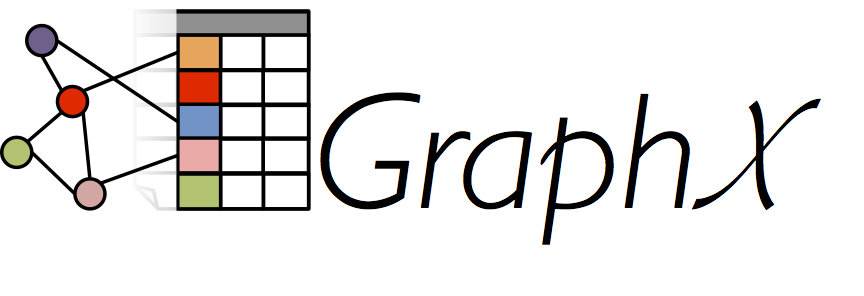
\includegraphics[width=.7\linewidth]{img/7-3_graphx.png}
        \caption{GraphX framework}
    \end{subfigure}%
    \caption{Stack of the different technologies we are using for the first solution}
\end{figure}

\subsection{Scala}

\footnotetext{\url{https://www.scala-lang.org/}}
\footnotetext{\url{https://en.wikipedia.org/wiki/Criticism_of_Java}}

Scala\footnotemark is a high-level programming language combining the object-oriented and functional paradigms. Intended to be concise and to answer the majority of Java's complaints.\footnotemark. Allowing operator overloading, a better functional support, lazy evaluation and requiring less boilerplate code. One of the features that I enjoy the most is pattern matching, which is not supported in Java. What's interesting is that Scala source code can be compiled into Java bytecode, the instruction set of the Java Virtual Machine. This way, a vast ecosystem of Java libraries are available when writing Scala programs. One of the main disadvantages of Scala is that major updates are not backwards compatible; this way, programs written in Scala 2.12 are not supported in 2.13. Not to mention that nowadays there exist two major branches of Scala development, namely Scala 2 and 3. Putting this all together, we can conclude that Scala is a bit unstable. A hell of a maintenance making loads of open-source projects and libraries get abandoned; we will discuss into this later on.

\begin{code}[Hello World written in Scala]
    \inputminted{scala}{code/listings/7-1_helloWorld.scala}
\end{code}

\subsection{Apache Spark}

Apache Spark is a Big data engine with support for several programming languages, including Scala and Python. Aiming to be simple, fast and scalable, it is the most widely-used engine in the industry. The idea behind Spark is creating a Framework that makes parallel jobs over high-volumes of data easy to write. It also bundles an engine supporting query optimization which will be discussed later on. For us to understand how Spark works, let's describe its architecture first. It follows the master-slave architecture, same idea behind the Pregel model, built on top of two abstractions, namely Resilient Distributed Dataset (RDD) and Directed Acyclic Graph (DAG).

\subsubsection{RDDs (Resilient Distributed Datasets)}

We want to process graphs in parallel, hence a distributed approach is required to store the graph itself. RDDs are necessary for us to address that issue. They are spread in memory or across several machines in a cluster, and serve as Apache Spark's primary logical data unit. This method allows a single RDD to be split into numerous logical segments that can then be stored and processed on various cluster machines. RDDs are also lazy-evaluated, which saves time and boosts efficiency. For us to have a better understanding of RDDs, their main features are listed below:

\begin{itemize}
    \item \textbf{Resilience or Fault tolerance:} RDDs keep track of data lineage information to automatically restore lost data in the case of failure.
    \item \textbf{Partitioning:} Any existing RDD can be partitioned to generate mutable logical sections. This can be done by performing transformations on the current partitions.
    \item \textbf{Lazy-evaluation:} Even if you define data, it does not load in an RDD. When you call an operation, like count or collect, or when you save the output to a file system, transformations are really computed.
    \item \textbf{Immutability:} You cannot alter the data that is saved in an RDD since it is in read-only mode. But by applying modifications to the current RDDs, you can produce new RDDs.
    \item \textbf{In-memory computation:} In order to allow faster access, an RDD stores every immediately created data in main memory.
\end{itemize}

After reviewing the key aspects of RDDs, let us try to improve our understanding by describing the environment that supports this abstraction. As stated in the introduction, Spark is constructed on top of RDDs; this includes abstractions such as DataFrames and Datasets which are developed on top of them.  Every computation in Spark is carried out by RDDs under the hood. In other words, these are Spark's most basic building blocks. Some advantages of the RDDs are their simplicity, capacity to import data from heterogeneous sources, ease of caching, and the ability to apply transformations to the data stored in a functional manner. However, as we are essentially storing Java objects (or Scala ones), they consume rather large amounts of memory, garbage collection is necessary, and serialization is required for data storage and retrieval. This issue is especially critical for larger datasets since the time to serialize/deserialize grows in proportion to the amount of data stored. More into this will be discussed later on.

\subsubsection{DAG (Directed Acyclic Graph)}

The main difference between Spark and Hadoop MapReduce, whose limitations lead to the creation of the former, is the DAG Scheduler. In the context of Apache Spark, a Directed Acyclic Graph, DAG for short, is a set of Vertices, representing an RDD partition, and the Edges, representing the operations to be applied. This graph is later transformed into stages by the DAG Scheduler, where each stage contains a series of tasks to be executed in parallel. As we had seen in section \ref{section:mapReduce}, the main issue with MapReduce is having to store the result of each intermediate node, in a DAG architecture this is not required.

\begin{figure}[ht]
    \centering
    \includestandalone[width=0.65\textwidth]{diagrams/7-1_apacheSparkArchitecture}
    \caption[Architecture of Apache Spark]{Architecture of Apache Spark\footnotemark}
    \label{fig:architecture:apacheSpark}
\end{figure}

\footnotetext{\url{https://spark.apache.org/docs/0.9.1/cluster-overview.html}}

\subsection{GraphX}

A graph processing framework integrated with Apache Spark was suggested as GraphX in 2014. Its API contains a Pregel variation that is used to implement several algorithms, including PageRank. GraphX exposes an API for graphs based on RDDs~\cite{https://doi.org/10.48550/arxiv.2110.11709}.

\subsubsection{The GraphX implementation of Pregel}

GraphX provides several built-in operators for graphs\footnote{\url{https://spark.apache.org/docs/latest/graphx-programming-guide.html\#graph-operators}}. We will use the following in the rest of the paper:

\begin{itemize}
    \setlength\itemsep{1em}
    \item \mintinline[fontsize=\small]{scala}{mapVertices(g: Graph[|\VertSet|,|\EdgeSet|], f: (Id,|\VertSet|)|$\rightarrow$||\VertSet|)): Graph[|\VertSet|,|\EdgeSet|]}
          \begin{itemize}
              \item[$\blacksquare$] \textbf{Description:} Transforms each vertex attribute in the graph using the map function. It maps every pair \texttt{(id,v)} -- which are the vertices of \texttt{g} -- into \texttt{(id,f(v))}.
              \item[!] \textbf{Note:} The new graph has the same structure. As a consequence the underlying index structures can be reused.
          \end{itemize}
    \item \mintinline[fontsize=\small]{scala}{mapReduceTriplets(g: Graph[|\VertSet|,|\EdgeSet|], m: (|\VertSet|,|\EdgeSet|,|\VertSet|)|$\rightarrow$|(Id,|\MsgSet|)), r: (|\MsgSet|,|\MsgSet|)|$\rightarrow$||\MsgSet|)): RDD[Id,|\MsgSet|]}
          \begin{itemize}
              \item[$\blacksquare$] \textbf{Description:} Takes a user defined map function \texttt{m} which is applied to each triplet and can yield messages which are aggregated using the reduce function \texttt{r}.
          \end{itemize}
    \item \mintinline[fontsize=\small]{scala}{joinVertices(g: Graph[|\VertSet|,|\EdgeSet|], msgs: RDD[Id,|\MsgSet|], f: (Id,|\VertSet|,|\MsgSet|)|$\rightarrow$||\VertSet|)): Graph[|\VertSet|,|\EdgeSet|]}
          \begin{itemize}
              \item[$\blacksquare$] \textbf{Description:} Joins the vertices with the input RDD and returns a new graph with the vertex properties obtained by applying the user defined map function to the result of the joined vertices. Vertices without a matching value in the RDD retain their original value.
          \end{itemize}
\end{itemize}

The GraphX Pregel implementation is defined iteratively where each iteration is usually called a superstep, taking as input a \texttt{Graph}[\VertSet, \EdgeSet] and the following parameters:

\begin{itemize}
    \item \texttt{initialMsg}: the message each vertex will receive at the initial iteration.
    \item \texttt{vProg}: the user-defined vertex program function which is ran on each vertex and computes a new value for it. During the first iteration, the vProg is invoked on all vertices. On subsequent iterations it is invoked only on those active vertices; that is, those receiving messages.
    \item \texttt{sendMsg}: the user-defined function that is applied to all the out edges of vertices receiving a message in the current iteration. That is, a function which computes the messages to be sent to the neighbors of a node for the next iteration.
    \item \texttt{mergeMsg}: the user-defined function that is applied to two incoming messages and merges them into one.
\end{itemize}

\begin{pseudocode}[The Pregel model as implemented in GraphX]
    \includestandalone{code/algorithms/7-1_pregel}
\end{pseudocode}

It is worth noting that the Pregel operator in GraphX is a \textit{bulk-synchronous} parallel messaging abstraction at a high level. The Pregel operator performs a sequence of supersteps in which vertices receive their inbound message set, calculate a new value for the vertex, and then send messages to their neighbors. Take a look at the first two lines of the pseudo-code above to see how the initial messages for each vertex are received and calculated for iteration 0. Messages, unlike Pregel, are calculated concurrently: note the second and fifth lines of the above snippet. Vertices that receive no messages are skipped. The Pregel operator ends iteration and returns the final graph when there are no messages left, as seen in the third line of the snippet above. The previously described constraints allow GraphX to perform some additional optimization.

\section{PSchema: ShEx + Pregel generated subsets}

The next paragraphs will provide a description of the ShEx validation algorithm based on Pregel. This approach is based on the assumption that a ShEx schema $\psi \mathcal{L},\sigma \psi$ is provided,  with each label $l \in \mathcal{L}$ identifying a shape expression.

According to the figure \ref{fig:state:pregel}, nodes might be active if they have received some messages, or inactive if they have not received any messages. Certain sub-states are necessary for us to produce a more accurate answer based on Knowledge graph validation. The algorithm in the Pregel approach is in charge of annotating each node $n\in\mathcal{V}$ with a status map expressing the validation status for specific labels.

\begin{figure}[H]
    \centering
    \includestandalone[width=0.66\textwidth]{diagrams/7-2_pregelState}
    \caption[State diagram representing the different states in \texttt{vProg}]{State diagram representing the different states in \texttt{vProg}~\cite{https://doi.org/10.48550/arxiv.2110.11709}}
    \label{fig:state:pregel}
\end{figure}

A more detailed description of the possible values that the \texttt{Status} can take is provided:

\begin{center}
    \begin{tabular}{ccll}
    $Status$ & ::=    & \texttt{Undefined}                  & Default status                                                         \\
             & $\mid$ & \texttt{Ok}                         & Node conforms to the schema                                            \\
             & $\mid$ & \texttt{Failed}                     & Node does not conform to the schema                                    \\
             & $\mid$ & \texttt{Pending}                    & Requested to be validated                                              \\
             & $\mid$ & \texttt{WaitingFor($ds$,$ok$,$fs$)} & Waiting for some neighbors                                             \\
             &        &                                     & $ds$ = list dependents neighbors                                       \\
             &        &                                     & $ok$ = list of conformant neighbors                                    \\
             &        &                                     & $fs$ = list of non conformant neighbors                                \\
             &        &                                     & where $ds$, $oks$, $failed$ $\in\VertSet\times\PropSet\times\LabelSet$
\end{tabular}
\end{center}

\begin{pseudocode}[Pregel-based ShEx validation pseudocode]
    \includestandalone{code/algorithms/7-2_pregelShEx}
\end{pseudocode}

\begin{table}
    \centering
    
\begin{tabular}{c}
    \inference[$$]
    {\fracEmpty{
            \msgSent{(n,m)}{\lbl}{\Validate}
        }{
            \status{m}{\lbl}=s\in\{\Undefined, \Pending\}
    }                                             & \checkLocal{\lbl}{n}=r\in\{\Ok,\Failed\}
    }
    {\status{m'}{\lbl}=r}

    \\ \\

    \inference[$$]
    {\fracEmpty{\msgSent{(n,m)}{\lbl}{\Validate}}
        {\status{m}{\lbl}=r\in\{\Undefined,\Pending\}
    }                                             & \checkLocal{\lbl}{n}=\PendingLs
    }
    {\fracEmpty{\status{m'}{l}=\Undefined}{\status{m'}{l'}=\Pending\,\,\forall{l'}\in{}ls}}

    \\ \\

    \inference[$$]
    {\fracEmpty{
            \msgSent{(n,m)}{\lbl}{\Validate}}
        {
            \status{m}{\lbl}=r\in\{\Ok,\Failed\}
        }
    }
    {\status{m'}{\lbl}=r}

    \\ \\
    % This is to stop the recursive case....if we request to validate a node for which we are already waiting for, we assume it is valid
    \inference[$$]
    {\fracEmpty{
            \msgSent{(n,m)}{\lbl}{\Validate}
        }{
            \status{m}{\lbl}=\WaitingFor{ds}{oks}{fs}
        }
    }
    {\status{m'}{\lbl}=\Ok}

    \\ \\

    \inference[$$]
    {\fracEmpty{
            \msgSent{(n,m)}{\lbl}{\Checked{oks}{fs}}}
        {
            \status{m}{\lbl}=\WaitingFor{ds}{oks'}{fs'}
    }                                             & ds\setminus(oks\cup{}fs)\neq{}\emptyset
    }
    {\status{m'}{\lbl}=\WaitingFor{ds}{oks\cup{}oks'}{fs\cup{}fs'}}

    \\ \\

    \inference[$$]
    {\fracEmpty{\msgSent{(n,m)}{\lbl}{\Checked{oks}{fs}}}
    {\status{m}{\lbl}=\WaitingFor{ds}{oks'}{fs'}} &
        ds\setminus(oks\cup{}fs)=\emptyset
    }
    {\status{m'}{\lbl}=\neighbors{\lbl}{oks\cup{}oks'}{fs\cup{}fs'}}
\end{tabular}\\


    \caption{Definition of \texttt{vProg} for Pregel-based ShEx validation}
\end{table}
\label{vProg}
\section{Evaluation of the solution}

As we have shown so far, the proposed solution is perfectly valid. Since the RDD-based API is based on the functional programming paradigm, the algorithm may be written using of higher-order functions. Takes the code readable even if you have no prior knowledge with Apache Spark. Moreover, as information is kept in the form of Java objects , the data flow is exposed in the same way that it is in any other Java application. This last argument becomes specially relevant when comparing it to DataFrame-based APIs, which are built on abstractions and a SQL engine. On the other hand, the memory usage is far from optimum in RDD-based solutions. The operations to be performed become less efficient as we must serialize and deserialize the data at each iteration of the algorithm. Not to mention the lack of a query execution optimizer, as well as the lack of data homogeneity due to RDDs' being schema-less. When everything is considered together, it is clear that there is a lot of room for improvement.

\chapter{Refactoring the Pregel-based algorithm}
\label{chapter:refactoring}
\epigraph{\textit{The business changes. The technology changes. The team changes. The team members change. The problem isn't change, per se, because change is going to happen; the problem, rather, is the inability to cope with change when it comes.}}{-- \textup{Kent Beck}}

During the early stages of the development, the first steps we followed were highly related to polishing and improving the solution described in the previous chapter. This was a challenging problem that resulted in a change in the project's direction, which will be detailed later.

\section{Technology stack}

As I mentioned earlier, the purpose of this second solution was to improve what was already implemented. This way, we kept most of the stack untouched. The sole change was the replacement of GraphX with its DataFrame equivalent library named GraphFrames.

\begin{figure}[ht]
    \centering
    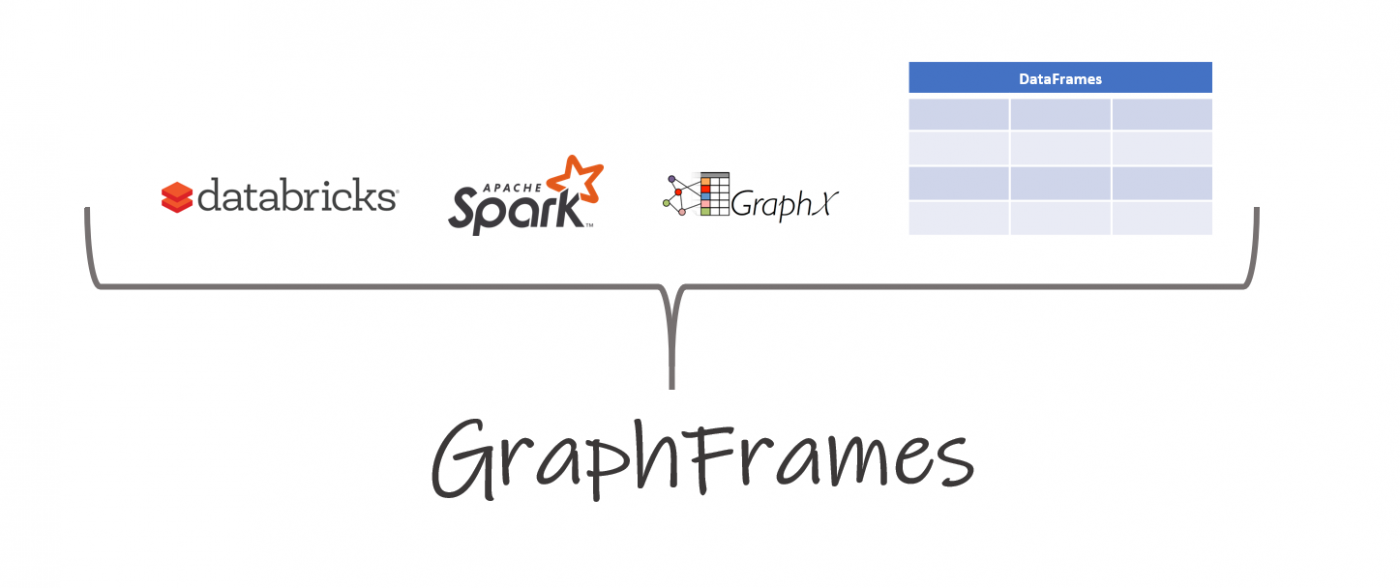
\includegraphics[width=.7\linewidth]{img/8-1_graphframes.png}
    \caption[Stack of the different technologies we are using for the second solution]{Stack of the different technologies we are using for the second solution\footnotemark}
\end{figure}

\footnotetext{\url{https://adatis.co.uk/graphframes/}}

\subsection{GraphFrames}

As it name goes, GraphFrame is a package for Apache Spark providing support for DataFrame-based Graphs. According to the introductory lines, the main goal of this stage of the development was to move our solution one step further in the abstraction level, from a solution based on RDDs to another based on DataFrames. From the ground up, we always believed RDDs weren't the go-to. What's more, RDDs are discouraged as they seem to be outdated in comparison to DataFrames and Datasets. More into this will be discussed in the next section. According to the description for GraphFrames, this API is similar to GraphX, except instead of being built on top of RDDs, they are built on DataFrames. The fact that the GraphFrames API for the Pregel algorithm has not been updated since 2018 makes us cautious of this approach.

\subsection{DataFrames and Datasets}

From Spark version 1.3 onwards, what were once known as SchemaRDDs are now referred to as DataFrames. That may give us an idea of what a DataFrame is. In that sense, they basically are RDDs provided some Schema for the data that is collected. With the help of this schema, DataFrames may be seen as rows with uniform structure: columns. Whereas RDDs are more akin to objects, DataFrames are closer to a table in a data base. This is quite relevant, as managing schemas to describe data allows us to perform operations over data in a much more efficient way than using Java serialization. It is worth mentioning that from Spark version 2.0 onwards, DataFrames can be understood as a type alias for \texttt{Dataset[Row]}, as they merged both APIs. In that sense, Datasets can be seen as the combination of the best from both worlds: with the appearance of a Java object from the outside, but with the shape of a table in RDBMS internally.

We now have a clear vision of what a DataFrame is. The problem is that even though they provide some nice features for data wrangling: schemas allow us to establish contracts so consumers know exactly the shape of the data they are working with, they are not so nicely implemented currently. Not only Apache Spark has no official support for working with DataFrame-based Graphs: notice GraphFrames is required, but the variety of supported types is scarce: including primitive types and Dates. Long has been discussed in this sense, but nothing has really changed since 2015\footnote{\url{https://issues.apache.org/jira/browse/SPARK-7768}}. To clarify this, let's put it into perspective.

\subsubsection{Encoders and User-defined Types}

% TODO: mention why Java serialization is so bad
% https://adtmag.com/articles/2018/05/30/java-serialization.aspx#:~:text=Serialization%20is%20brittle%2C%20it%20pokes,motivated%20getting%20it%20in%20there.

Working with simple data-structures is a trivial task in Apache Spark. What is not so easy to handle are custom data types. If the DataFrame cannot implicitly retrieve an Encoder, the user will be required to provide one. This is needed for Spark SQL to infer the schemas of the data we are working with. The complex the data-structure, the harder it is for the programmer to write an appropriate serialization/deserialization mechanism. Notice how this solution is far from efficient as it is based on serialization for data storage and retrieval, something we were trying to fix from the RDD-based solution. Another possibility could be writing your own User-defined type, which can be understood as a wrapper for the actual type. However, the amount of boiler-plate code needed, and the complexity of the data to be stored prevents us from writing an appropriate solution. More into this will be discussed in the following paragraphs.

% TODO: check what has been written here

As we have mentioned earlier, two main possible solutions arise for the problem of handling complex data: \textit{Custom encoders} and \textit{User-defined types}. It is a requirement for this solution not only to handle complex data, but unsupported, as we are not only trying to store complex data structures, but types that are not currently supported by the DataFrame API. This is a crucial argument against this DataFrame-based solution as we need to store URLs, which aren't supported by Spark SQL. The problem is that both of the mentioned solutions are inefficient. First, collection Encoders tend to act as bottlenecks in terms of performance. To follow up on this, storing non-standard objects in Spark is a mess\footnote{\url{https://stackoverflow.com/questions/36648128/how-to-store-custom-objects-in-dataset}}. The current situation of the Framework basically supports primitive types and not so complex case classes. The currently accepted solution in this sense consists of serializing objects using the \texttt{kryo} encoder which stores them as flat binary objects, preventing us from accessing concrete columns without deserializing the binary object. This last matter is specially crucial as messaging in Pregel is built on top of aggregates over particular columns. Hence, for each iteration we would need to serializing and deserialize every object stored. Thus, a custom, complex and inefficient encoder or type is not the solution we need. See figure \ref{fig:wikibaseClassDiagram} for an expanded description of the data model we are working with.

As a remark, it is worth noting that the code implementing the User-defined types for the data model above has a length of around 700 lines of code. While the actual algorithm takes around 100 lines of code to be written. For us to understand this, we have to describe how the so-called User-defined types are implemented in Apache Spark.

\begin{code}[User-defined types as implemented in Apache Spark]
    \inputminted{scala}{code/listings/8-1_udt.scala}
\end{code}

As noted in the first line of the above example, the description of user-defined types is annotated as an unstable API meant for developers. This implies that in minor Spark versions, the API may change or be eliminated. The use of it is at the user's own risk. As a consequence, if we follow this approach, we will end up with an unstable solution. Not only that but the processes for serializing and deserializing, along with the SQL schema -- which is no longer inferred by Scala's reflection system -- should be explicitly defined. Having said that, after we've specified what we've covered above, we're only establishing the wrapper, and yet no relationship is established between the real object and the User-defined type in the eyes of Spark's engine. To deal with this, we have two options: annotating the class we want to encapsulate or explicitly registering it. The former requires that the programmer has access to the class being wrapped. An ineffective technique that has been superseded by the latter since Spark 2.0. What's striking here is that it took Spark developers 6 years to come up with an answer in this regard. The API for user-defined types is essentially unmaintained, and dealing with custom objects in Spark is the framework's weak point. More on this was covered in the previously mentioned issue\footnote{\url{https://issues.apache.org/jira/browse/SPARK-7768}}.

\begin{code}[Registration of an User-defined type in Apache Spark]
    \inputminted{scala}{code/listings/8-2_udtRegistration.scala}
\end{code}

The issue here is the complexity of the data structures we use. According to the design in figure \ref{fig:wikibaseClassDiagram}, storing both \texttt{Statements} and \texttt{Entities} presents two major challenges. To begin, because the items stored require a fixed structure and we would like to polymorphically treat \texttt{Properties} and \texttt{Items} -- both -- as \texttt{Entities}, we need a mapping to convert from an object-oriented model to the relational paradigm. In this regard, we suggest \textit{Single Table Inheritance}\footnote{\url{https://en.wikipedia.org/wiki/Single_Table_Inheritance}}; that is, using a single table containing all the fields of all the child classes. The drawback is that we would end up with a solution in which rows contain redundant data: as many \texttt{NULL} values as different fields in child classes which are not the actual type for a certain row. Although it is a straightforward approach, it is inefficient. Second, this technique leads to a circular dependency\footnote{\url{https://en.wikipedia.org/wiki/Circular_dependency}} in which \texttt{Entities} include many \texttt{LocalStatements} that hold \texttt{Qualifiers} that may enclose \texttt{Entities}. When you define a schema for this problem, you eventually wind yourself in an infinite recursion where \texttt{Entities} have \texttt{Entities}. In conclusion, User-defined types offer a poor solution that causes several challenging issues.

\begin{figure}[ht]
    \centering
    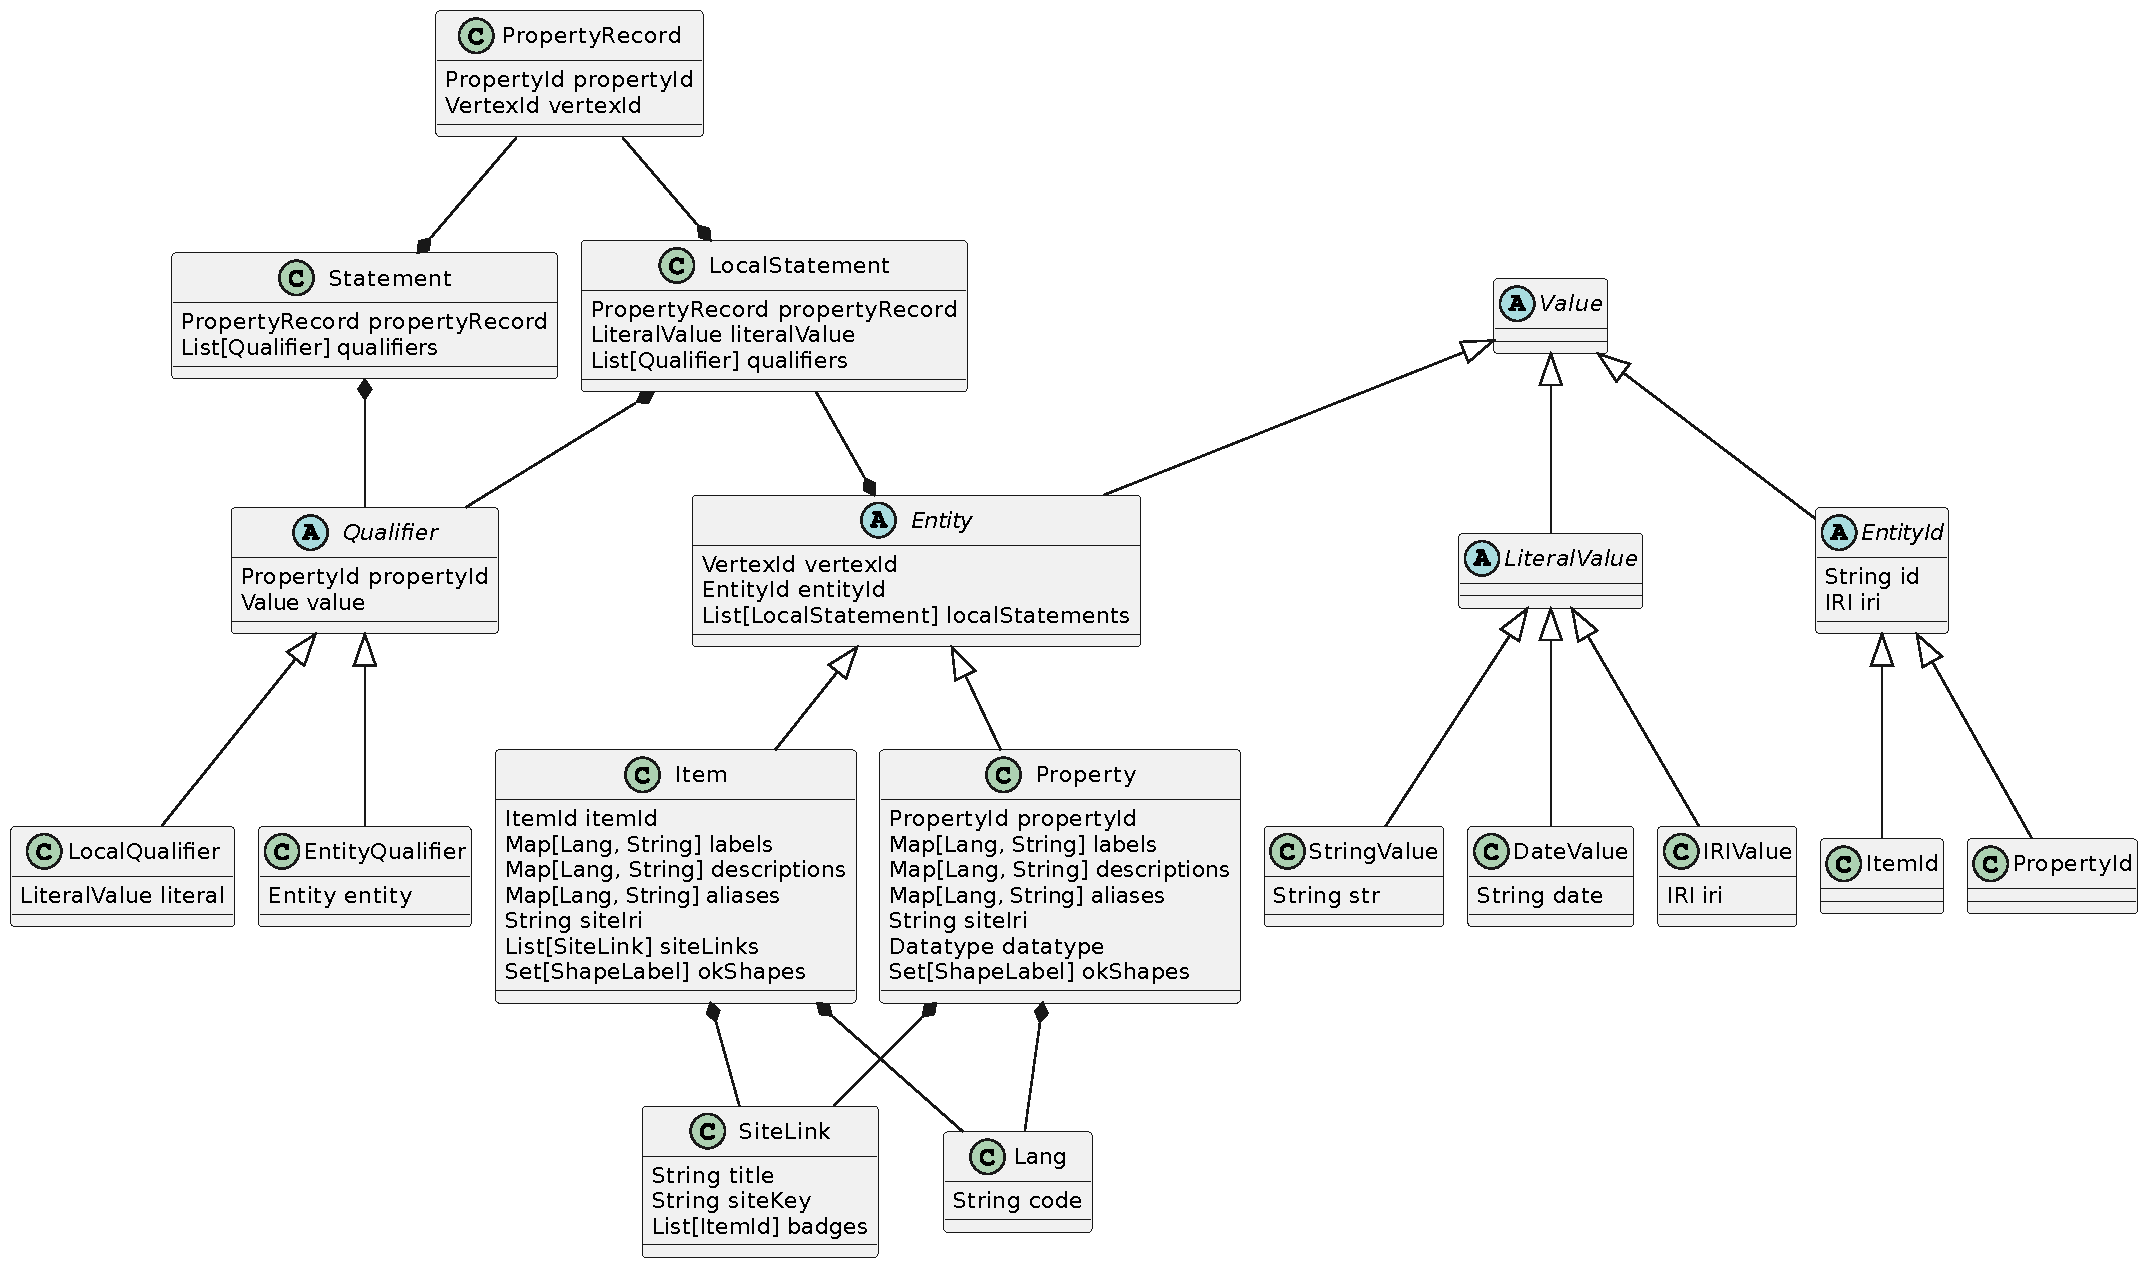
\includegraphics[width=\textwidth]{diagrams/8-1_wikibaseClassDiagram.pdf}
    \caption[Class diagram of the Wikibase data model as implemented in WShEx]{Class diagram of the Wikibase data model as implemented in WShEx\footnotemark}
    \label{fig:wikibaseClassDiagram}
\end{figure}
\footnotetext{\url{https://github.com/weso/shex-s}}

\part{Is Distributed Computing the solution?}

\chapter{Analysis of the Rust solution}
\label{chapter:analysis}
\epigraph{\textit{The most damaging phrase in the English language is "we have always done it this way".}}{-- \textup{Grace Hopper}}

We have examined two distinct Scala and Apache Spark-based solutions up to this point. Both were, as we have mentioned, far from ideal. We have to start from scratch if we want to find a more sophisticated solution.

\section{Technology stack}

\begin{figure}[ht]
    \centering
    \newsavebox\mybox
    \savebox{\mybox}{
\includegraphics[width=.3\linewidth]{img/9-1_rust.jpg}}
    \begin{subfigure}{.3\textwidth}
        \centering
        \usebox{\mybox}
        \caption{Rust programming language}
    \end{subfigure}%
    \hspace*{0.1em}
    \begin{subfigure}{.3\textwidth}
        \centering
        \vbox to \ht\mybox{%
            \vfill
            
\includegraphics[width=.9\linewidth]{img/9-2_duckdb.png}
            \vfill
        }
        \caption{DuckDB}
    \end{subfigure}%
    \hspace*{0.1em}
    \begin{subfigure}{.3\textwidth}
        \centering
        \vbox to \ht\mybox{%
            \vfill
            
\includegraphics[width=.8\linewidth]{img/9-3_polars.pdf}
            \vfill
        }
        \caption{Pola-rs}
    \end{subfigure}%
    \caption{Stack of the different technologies we are using for the third solution}
\end{figure}

\subsection{Rust}

Rust is a multi-purpose and high-level programming language. Its primary focus is on performance, memory safety, and concurrency. In this perspective, Rust might be considered a modern language, and as of March 18th, 2023, the most recent stable release is version 1.68. For achieving memory safety and concurrency, both at the same time, Rust prevents data races through a \textit{borrow checker} that tracks the object and allows each memory position to have only one owner at a time. Rust is popular for systems programming, and was included by the Linux kernel in December 2022, but it also has some high-level functional constructs like pattern-matching and the neatly implemented \texttt{Enums}.

The key features of Rust are:

\begin{enumerate}
    \itemsep0.5em
    \item \textbf{Performance:} It accomplishes this by employing a static memory management strategy rather than a garbage collector, using \textit{ownership} instead. This means that the compiler decides when memory is allocated and released at compile time. Rust can produce incredibly effective code as a result.
    \item \textbf{Memory safety:} Rust is designed to be memory safe. It achieves this by using a \textit{borrow checker}. This means that the compiler determines at compile time when memory is accessed, allowing Rust to prevent memory issues like use-after-free and double-free.
    \item \textbf{Concurrency:} Rust is designed to be \textit{concurrent}. This means that Rust programs can be executed in partial order, or out-of-order, without affecting the outcome. This allows the parallel execution of the concurrent units, significantly increasing the performance of the program in multi-threaded systems.
\end{enumerate}

An example of a simple \textit{Hello World} program written in Rust is shown below.

\begin{code}[Hello World written in Rust]
    \inputminted{rust}{code/listings/9-1_helloWorld.rs}
\end{code}

Having that said, let me make a brief remark on some of the features that I loved the most when working with Rust. Regarding the compiler, first of all, it is very strict and will not allow you to compile your code if it is not safe. This is a great feature because it will prevent you from having to deal with runtime errors. Secondly, the compiler is very helpful and will give you a lot of information about the error that you are facing. This is, it will help you to understand what is going on and how to fix it. Lastly, the compiler is very smart and will optimize your code for you. This is a great feature because it makes you write code that is fast and efficient, without even realizing it.

Regarding the language itself, first of all, Rust is heavily inspired by functional programming languages. Hence, many of the features that you will find in Rust are also present in Scala. Recall that one of the features that I loved the most about the latter was \textit{pattern matching} and Rust has it too. Secondly, Rust has a very powerful type system. What I enjoy about this feature is the way Rust handles errors. This is, by returning either a \texttt{Result} or an \texttt{Option} type, Rust forces you to handle errors and nullable functions safely. When combined with the \texttt{?} operator, error handling becomes very easy and concise. What's more, you can manage both through the \texttt{match} statement, a really clean approach. Lastly, concurrency is implemented following the same design principles as in Go, that is, it adheres to the \textit{share memory by communicating} principle: \textit{Do not communicate by sharing memory; instead, share memory by communicating}. This means that Rust uses \textit{channels} to communicate between threads, which is a very safe and efficient way of doing it. Rust's concurrency system reminds me of the idea behind the Pregel model, where the data is partitioned and sent to the different workers, which are the threads in this case. Then, workers can communicate with each other through the channels, which is the same as sending messages between workers in the Pregel model.

\subsection{DuckDB}

Conversely, DuckDB is an in-process SQL OLAP database management system written in C++ that is intended to be integrated into other applications. This means that DuckDB follows the ACID model and supports popular SQL constructs like window functions, table expressions, and JSON. Additionally, it is column-oriented storage and was created with analytical queries in mind. The impact of this last remark on the scope of our project will be explained further below. Being a project that is only a few years old, DuckDB is still being actively developed.

The key features of DuckDB are:

\begin{enumerate}
    \itemsep0.5em
    \item \textbf{In-process:} DuckDB is an embedded database that runs in the same process as the application. This means that there is no separate server process that needs to be started, stopped, or configured. The application can directly interact with DuckDB via a C API. Notably, this API is designed to be identical to the one utilized by SQLite. As a result, DuckDB can seamlessly substitute SQLite as a plug-and-play alternative.
    \item \textbf{OLAP or On-Line Analytical Processing:} DuckDB is designed for OLAP workloads. It is optimized for analytical queries that scan large amounts of data and perform complex aggregations. This is in contrast to OLTP, or On-Line Transaction Processing, which is optimized for transactional workloads with a high number of small transactions. DuckDB is not a suitable replacement for a traditional OLTP database like PostgreSQL or MySQL.
    \item \textbf{Columnar:} DuckDB is a columnar database. This means that data is stored in columns instead of rows. This can dramatically minimize the amount of data that needs to be read from memory because DuckDB can now only read the columns needed for a query. The vectorized query execution method, which enables incredibly quick query execution, benefits from the column orientation as well. Last but not least, the compression efficiency of the columnar storage format can help to further reduce the quantity of data that needs to be read from memory.
\end{enumerate}

\subsection{Pola-rs}

Pola-rs is a fast and memory-efficient DataFrame library for Rust. It is built on top of Apache Arrow, a cross-language development platform for in-memory data. This means that data can be shared between languages without the need for serialization or deserialization. Many well-known data science and analytics frameworks, such as Apache Parquet, Apache Spark, Dask, and Pola-rs, employ Apache Arrow. Putting it all together, Pola-rs is a DataFrame implementation written in Rust, a data structure that is commonly used in data science and analytics.

The key features of Pola-rs are:

\begin{enumerate}
    \itemsep0.5em
    \item \textbf{Zero-copy:} Pola-rs is a DataFrame library that uses Apache Arrow as the memory model. This means that Pola-rs does not copy data when performing operations on the DataFrame. Instead, it manipulates the metadata of the underlying Arrow array. This makes Pola-rs very fast and memory efficient.
    \item \textbf{Parallel execution:} Pola-rs is designed to be parallel. This means that Pola-rs can execute operations on several threads at the same time. This allows Pola-rs to take advantage of multi-core systems, resulting in faster execution.
    \item \textbf{Lazy evaluation:} Pola-rs is designed to be lazy. This means that Pola-rs does not execute operations until they are needed. This allows Pola-rs to avoid unnecessary computations, resulting in faster execution.
    \item \textbf{Query optimization:} Pola-rs' Lazy API optimizes the query plan for it to be executed faster. This means that Pola-rs can optimize queries by reordering operations and removing unnecessary ones. This allows queries to be executed faster.
    \item \textbf{Streaming:} Pola-rs is designed to allow streams from external files. This means that Pola-rs can process data in batches read from an external file or database. This allows Pola-rs to process data without having to load it all into memory first, resulting in the possibility of processing larger datasets, even if they do not fit in memory.
\end{enumerate}

\section{Extract-Transform-Load}

As discussed in the preceding chapter, we have encountered challenges related to the data model we are currently handling. The primary issue arises from the data's lack of a convenient structure for manipulation. Circular dependencies and recursive structures have proven to be problematic in our case. Consequently, we have decided to migrate the data to a relational database, which would provide a more organized and valid data model. The initial step involves extracting the data from the JSON file and transforming it into a format that facilitates seamless processing. This is where the Extract-Transform-Load (ETL) process becomes crucial.

The Extract-Transform-Load (ETL) process is a data integration method aiming at extracting data from one or more sources, transforming it, and loading the result into a target system. An ETL process is a critical component of data-intensive applications, as having properly structured and valid data has a strong impact on the quality of the results and the performance of the system. With that said, the ETL process is used in data migration projects, where data is moved from one system to another. This last remark is important because it is the case of our project, where we are willing to move data from a JSON file to a relational database.

\begin{figure}[ht]
    \centering
    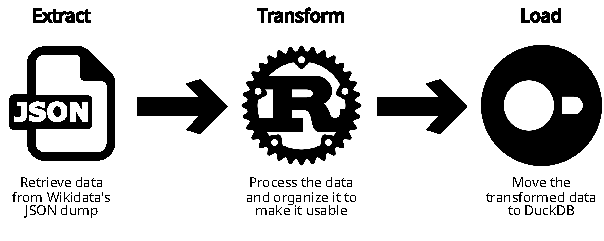
\includegraphics[width=0.8\textwidth]{diagrams/9-1_etl.pdf}
    \caption{Extract-Transform-Load (ETL) process description}
\end{figure}

\subsection{Extract}

The first step of the ETL process is the extraction of data from the source system. This step is responsible for connecting to the source system and retrieving the data. The source system can be a database, a file, or even a web service. In our case, we want to extract the data from a JSON dump, so we will need to connect to the file system and read the data from the file. See section \ref{section:json_dump} for more details.

\subsection{Transform}

The second step of the ETL process is the transformation of data. This step is responsible for converting the data from its source format to the target format. It is also responsible for cleaning the data, removing duplicates, and performing other operations to ensure that the data is valid and consistent. In our case, we want to transform the data from a JSON format to DuckDB. Not only that, but we also have to store the data in a way that is consistent with the knowledge graph model. This means that we have to extract the entities and relationships from the data and represent them in a graph format. See section \ref{section:wd2duckdb_design} for more details.

\subsection{Load}

The third and final step of the ETL process is the loading of data into the target system. It is responsible for connecting to the target system and inserting the data. In our case, we want to load the data into a DuckDB database. See section \ref{section:duckdb_load} for more details.

For us to accomplish what we have just described, we will need to use a tool that can perform the ETL process. In our case, we will implement one ourselves using Rust. This tool will be responsible for extracting data from a JSON file, transforming it into a relational format, and loading it into a DuckDB database. The tool will be called \texttt{wd2duckdb}. See chapter \ref{chapter:wd2duckdb} for more details.

\section{Knowledge Graph Subsets}

Moreover, merely having our data stored in a relational database is insufficient. It is crucial to remember that our objective is to develop an algorithm capable of validating Knowledge graphs. As a result, we must establish a system that allows us to query the graph in a Pregel-like manner. Currently, there is no existing implementation written in Rust and based on DataFrames that aligns with our requirements. Hence, we will introduce a new system called \texttt{pregel-rs} to fulfill this need. Additionally, we will also require an algorithm for generating subsets, which will be named \texttt{pschema-rs}. Further information can be found in Chapter \ref{chapter:pschema}.

\chapter{From Wikidata JSON dumps to DuckDB}
\label{chapter:wd2duckdb}
\epigraph{\textit{Information flow is what the Internet is about. Information sharing is power. If you don't share your ideas, smart people can't do anything about them, and you'll remain anonymous and powerless.}}{-- \textup{Vint Cerf}}

We have seen thus far the two main export formats supported by Wikidata, namely, RDF and JSON. However, none of them are suitable for analytical queries. In this chapter, we will explore the possibility of exporting Wikidata in a columnar format, as we have mentioned in the previous chapter, DuckDB is the perfect candidate for this task. This is, we will create a Rust-based solution for exporting Wikidata to DuckDB.

\section{The issue with JSON and other text-based formats}
\label{section:issue}

JSON is a text-based format, and as such, the data that is stored inside a JSON file is not compressed in any way. This means that the size of the file is directly proportional to the size of the data. This is not a problem for small datasets, but it becomes an issue when we are dealing with larger information repositories. As we have seen in the introductory chapter a Wikidata JSON dump is around \texttt{1.5 TB} in size when uncompressed. See Chapter \ref{chapter:intro} for a more detailed explanation. The challenge lies in the inability to load such a massive file into the memory of a single machine. Even if feasible, the loading process would be time-consuming and incur substantial expenses for renting a suitable machine. As a result, a binary format is required to store the information. This is where DuckDB comes into play. Despite the need to load the database into memory (recall, DuckDB is an in-process or embedded database), the repository's size is considerably smaller than that of the JSON file, often differing by several orders of magnitude. DuckDB achieves this by utilizing a columnar database structure, enabling more efficient compression of the data compared to a text-based format. This compression advantage is the primary reason driving our decision to export Wikidata to DuckDB.

It is worth mentioning that Wikidata JSON dumps follow a structure where each line of the file stores a single object. This provides the advantage of being able to parse the file line by line, which is quite convenient. However, there is a drawback: every line in the dump includes redundant boilerplate information related to the JSON object schema. In other words, we may have hundreds of millions of lines, all containing the same boilerplate code. Instead of having a header with the object schema, it is repeated in every line of the document. This redundancy significantly impacts the memory efficiency of JSON files. While JSON is excellent for sharing information, it is not the most efficient option for storage purposes.

\section{wd2duckdb}

Now that we have a clear understanding of the scope of the project, we can start working on the design of the tool in charge of transforming the Wikidata JSON dumps into a DuckDB file. For us to do so, some decisions are made. First, we are interested in storing only one of the translations of each Wikidata entity; that is, we are going to store only one of the labels, descriptions and aliases of each item. However, the language of choice can be modified\footnote{\url{https://github.com/angelip2303/wd2duckdb/blob/master/wikidata-rs/src/lib.rs\#L20}}. Second, we are going to store only the statements that are not deprecated. Apart from that, the rest of the information is going to be stored as it is.

\label{section:wd2duckdb_design}
\subsection{Design}

The tool is going to be divided into two main parts. The first one is going to be in charge of parsing the Wikidata JSON dump and extracting the information that we are interested in. The second part is going to be in charge of storing the information in a DuckDB database. The idea is to allow backends to be interchangeable; that is, several implementations for other drivers should be implemented without actually changing the existing code. However, for the sake of simplicity, we are going to focus on DuckDB for the time being.

\label{section:json_dump}
\subsubsection{Parsing the JSON dump}

The first part of the tool is going to be in charge of parsing the Wikidata JSON dump and extracting the information that we are interested in. In this manner, we are going to parse the JSON dump line by line. Recall, each line of the dump contains a single JSON object, which is -- indeed -- a Wikidata entity. It is worth noting that the entities in the array are not sorted in any way. This is, we have to be aware that the first entity in the dump is not necessarily the first Wikidata entity, namely, \texttt{Q1}. Thus, our solution should not rely on the order of the entities in the dump. What's more, a certain entity of the dump can refer to another that has not been parsed yet. Hence, we must be able to handle this situation as well.

Having that said, it is worth mentioning that a Wikidata dump can contain hundreds of millions of entities. This means that we cannot store all that information in memory. Hence, we must find a way to append the information to the resulting database as we parse the dump.

\label{section:duckdb_load}
\subsubsection{Storing the information in DuckDB}

The second part of the tool is going to be in charge of storing the information we have retrieved in the resulting database. Hence, we are going to load the following information into DuckDB:

\begin{itemize}
    \itemsep0.5em
    \item \textbf{Wikidata IDs}: As we had seen in section \ref{section:wikibase_graphs}, Wikidata IDs consist of a type prefix \texttt{Q}, \texttt{P} or \texttt{L}, for identifying Entities, Properties or Lexemes, followed by a sequence of numbers. There exist other two types of IDs, namely, \texttt{F} and \texttt{S}, for identifying Forms and Senses, respectively. A more detailed discussion on this topic will be presented later on.
    \item \textbf{Labels}: We are going to store the labels of the entities in the same table where we store the IDs.
    \item \textbf{Descriptions}: We are storing the descriptions of the entities in the same table where we store the IDs.
    \item \textbf{Statements}: We are going to store the statements of the entities in a separate table so that we can build the graph later on. The idea is to store the ID of the source entity, the ID of the property and the ID of the destination entity. In this manner, we will end up with two main tables: one for storing the entities, or vertices, and another one for storing the statements, or edges. Several other tables are going to be created for storing data relative to the information that comes with the statements, such as qualifiers, references, ranks, etc. However, for the time being, we are going to focus on the main tables.
\end{itemize}

According to what we have just described, we are going to end up with a database that contains two main tables: one for storing the entities, or vertices, and another one for storing the statements, or edges. The schema of the database is depicted in figure \ref{fig:schema}.

\begin{figure}[ht]
    \centering
    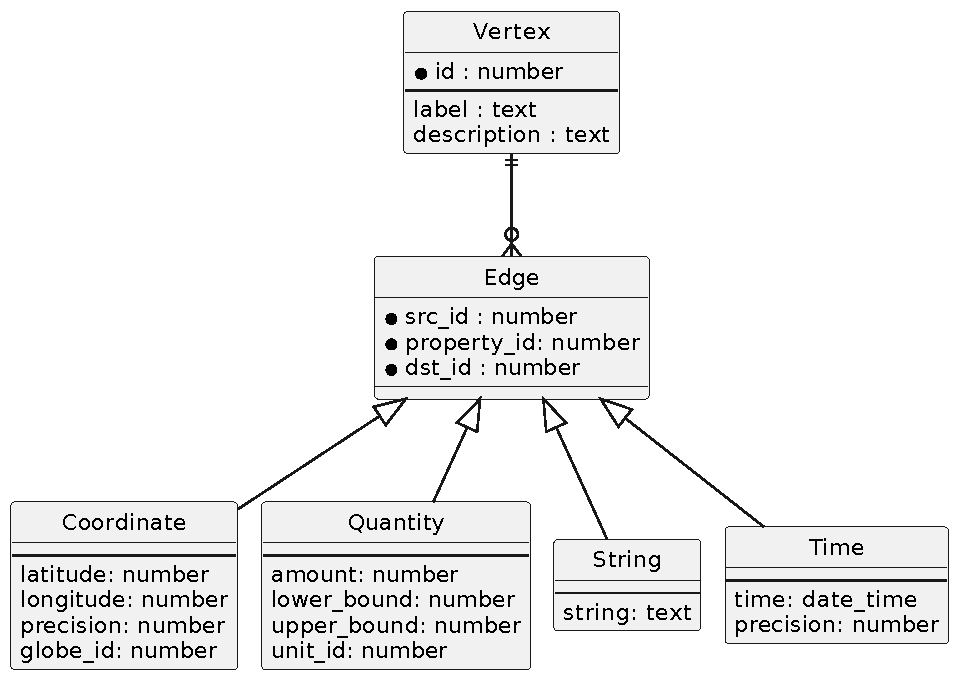
\includegraphics[width=.75\linewidth]{figures/diagrams/10-1_wd2duckdb.pdf}
    \caption{Entity-relationship diagram of the Database created by the \texttt{wd2duckdb} tool}
    \label{fig:schema}
\end{figure}%

\subsection{Implementation of the \texttt{wd2duckdb} tool}

Once we have a better understanding of the design of the tool. Now, we can start working on the implementation of it. The idea is to create a Rust-based solution that can be used as a library or as a command-line tool. This CLI will act as a wrapper for the library and is responsible for calling it, as well as handling command-line inputs such as the source JSON and the target file. Through \texttt{crates.io}\footnote{\url{https://crates.io/crates/wikidata-rs}}, we aim to make the library available to other Rust projects. This is, we are looking to decouple the library from the binary for other backends to be implemented on top of the same traits.

The most relevant aspect of the implementation revolves around the insertion of the processed Wikidata entities into the database. To accomplish this, we will leverage the powerful \texttt{duckdb-rs}\footnote{\url{https://crates.io/crates/duckdb}} library, which provides a Rust interface for DuckDB. Note that, it is based on the same interface as the SQLite driver for Rust. The plan is to utilize this library to create the necessary database and tables, and then employ it again to insert the data into it. The diagram in Figure \ref{fig:activity} illustrates the implementation of the \texttt{wd2duckdb} tool.

To insert the data into the database, we first need to establish a connection to it by creating a \texttt{Connection} object. Subsequently, we create the \texttt{Statement} and execute the corresponding SQL statement, specifically an insert one. However, the main concern arises executing the aforementioned statements for each entity, as it would severely impact the tool's performance due to the need for creating numerous connections to the database, corresponding to the number of lines in the JSON dump. To address this issue, we employ a transactional approach. By creating a transaction and executing the insert statements within it, we can greatly enhance the tool's performance. Once all the entities have been inserted, we commit the transaction. Notably, this approach requires only a single connection to the database. It becomes even more convenient when utilizing the \texttt{duckdb-rs} library, as it provides an \texttt{Appender} struct. The \texttt{Appender} not only encapsulates the transaction but also optimizes the data insertion process by buffering the data and inserting it into the database in batches. Consequently, the tool's performance is further improved. This is the recommended approach for inserting large amounts of data into a database.

\begin{figure}[p]
    \centering
    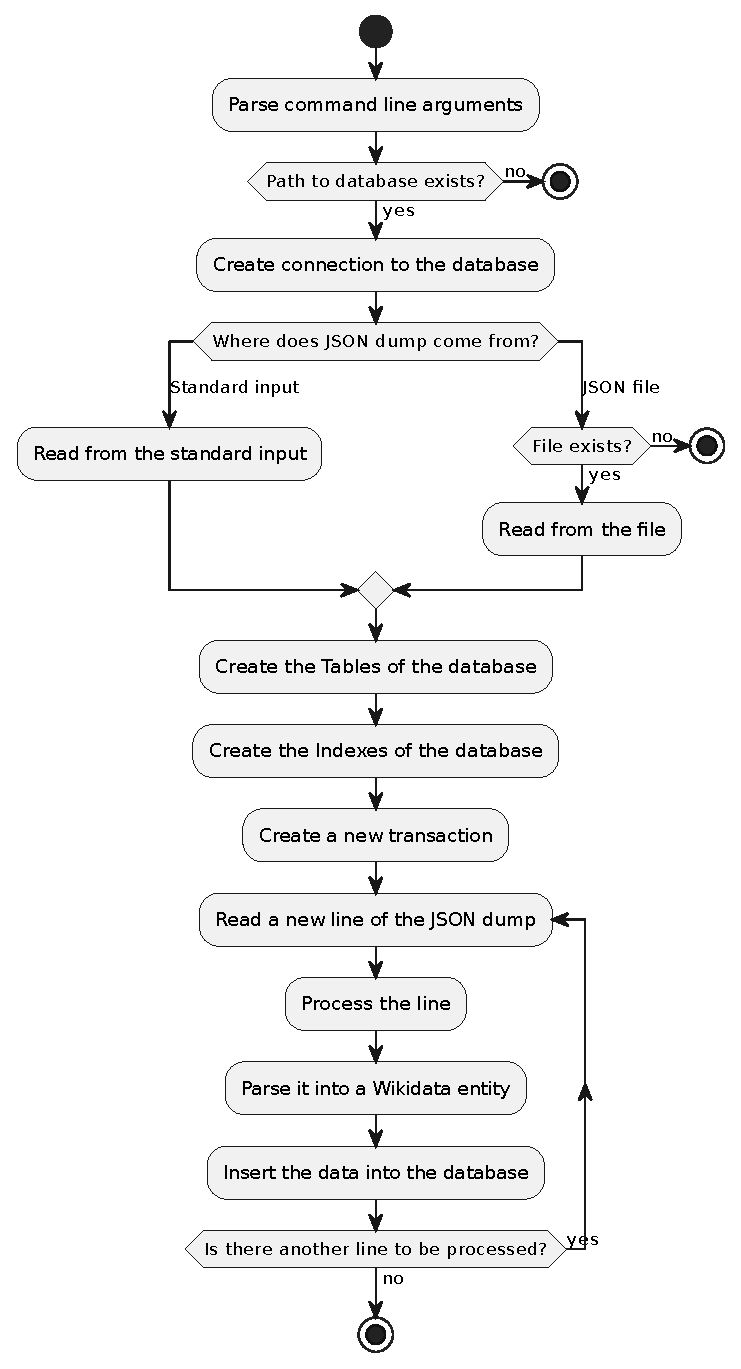
\includegraphics[width=.66\linewidth]{figures/diagrams/10-2_wd2duckdb.pdf}
    \caption{Activity diagram of the \texttt{wd2duckdb} tool}
    \label{fig:activity}
\end{figure}%

\subsection{Optimizations}

The Wikidata JSON dump is a huge file. As we have seen in section \ref{section:issue}, it is around \texttt{1.5 TB} in size. This means that we need to put an extra effort into optimizing the tool. For that, we are going to use a combination of different techniques, such as compression, and fine-tuning the chosen data types.

\subsubsection{Compression}

Dealing with large amounts of data is far from being trivial. For that, we are going to use compression techniques to reduce the size of the data that we are going to store. Those mechanisms can potentially reduce the size of the data by a factor of 10. This is not only beneficial for reducing the storage footprint, but it also helps improve the performance of tools consuming the data as fewer reads from disk or over a network connection are required. Column store formats are known for being highly compressible, and DuckDB is not an exception. This is because data within a column tends to be similar to each other, which is not the case for row-based formats, where each row is composed of heterogeneous data types, leading to lower compression rates.

The best thing about compression in DuckDB is that it will automatically choose the better compression algorithm for us \cite{Raasveldt_2022}. This is because it can detect the data type of each column, and based on that, it will choose the best compression method. For example, DuckDB will probably choose \texttt{RLE or Run-length encoding} for storing the identifiers of the properties, as it decomposes the dataset into pairs of (value, count) tuples, where the count represents how many times the value is repeated. Thus, no repeated values are stored. This is useful as several different entities may claim the same property, such as \texttt{P31} (instance of), where almost every Wikidata item will have it. Hence, we can take advantage of this and compress the data using \texttt{RLE}. To put it in a nutshell, \texttt{RLE} is a lossless compression algorithm that replaces repeated values with a single value and a count. This is illustrated in figure \ref{fig:rle}.

\begin{figure}[ht]
    \centering
    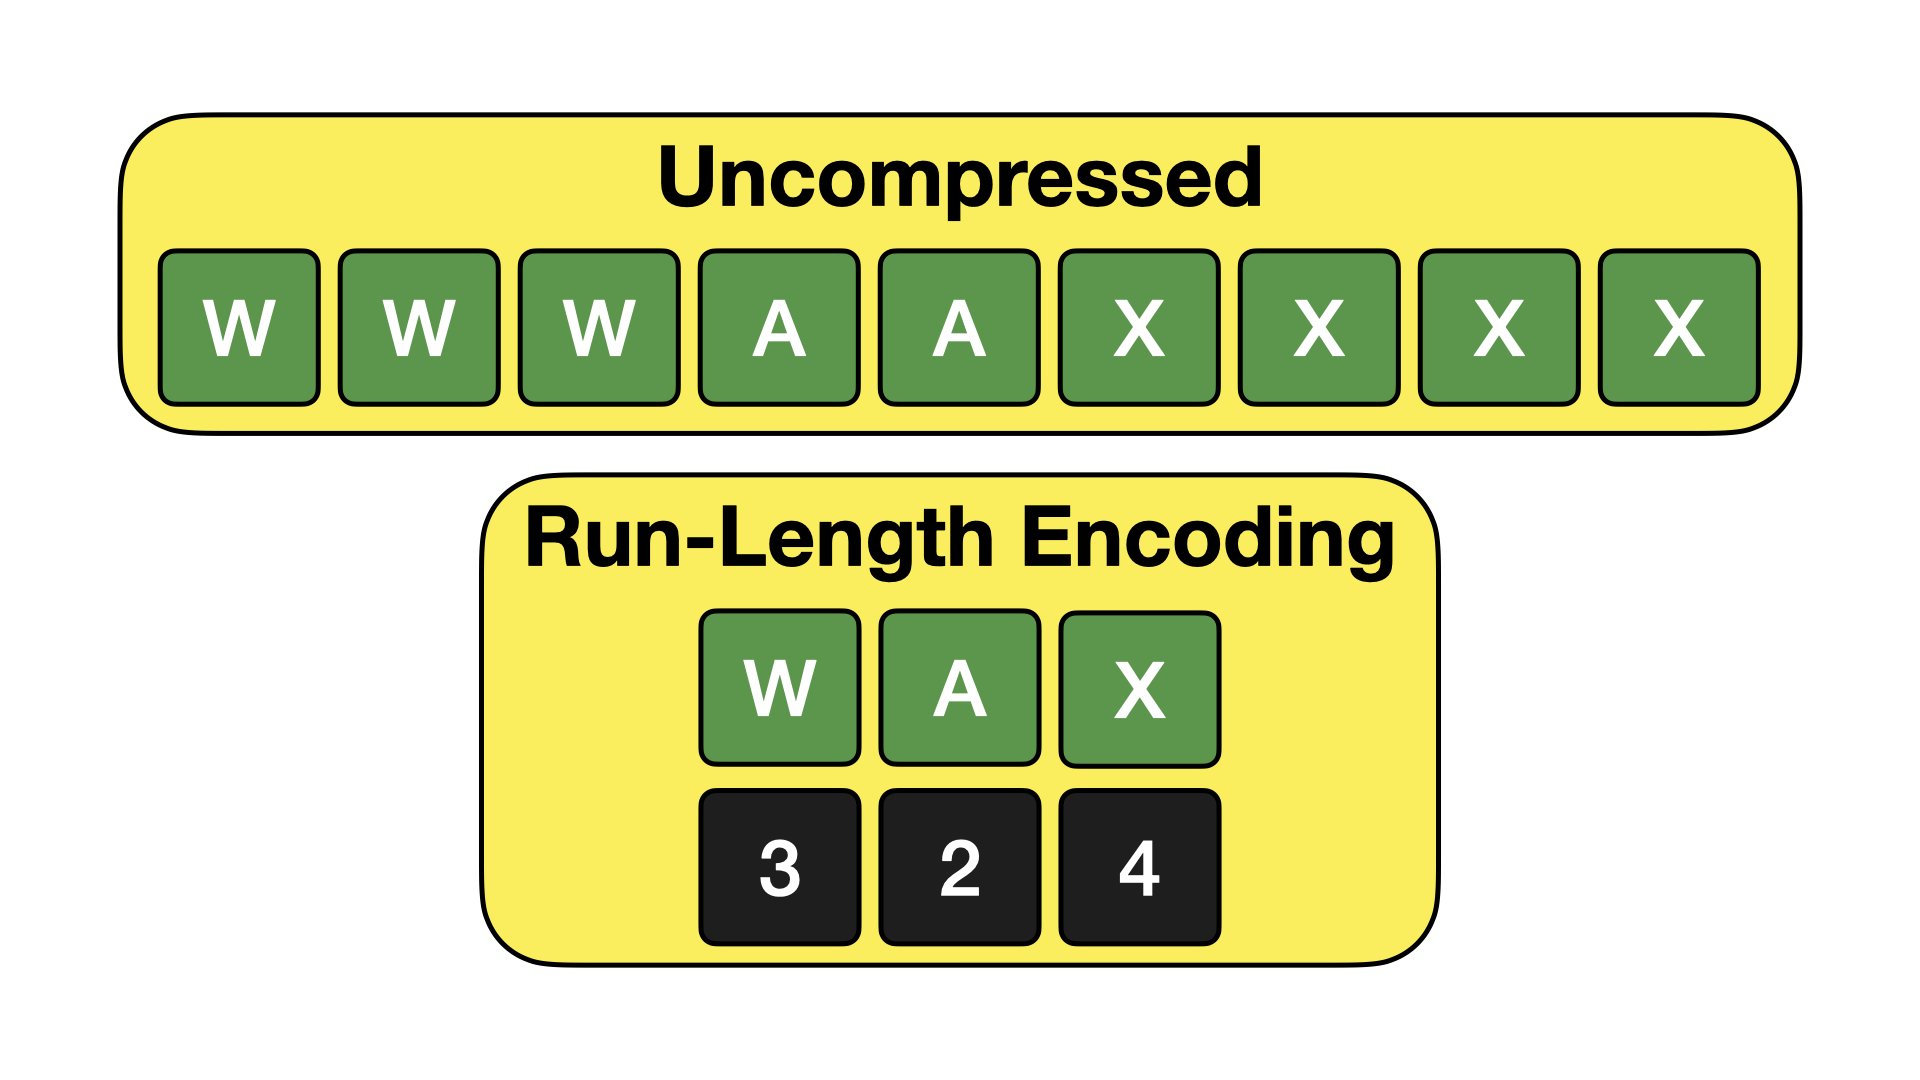
\includegraphics[width=.8\linewidth]{figures/diagrams/10-2_rle.png}
    \caption[Example of \texttt{RLE} compression]{Example of \texttt{RLE} compression \cite{Raasveldt_2022}}
    \label{fig:rle}
\end{figure}

In the given example, the original sequence \texttt{WWWAAXXXX} is compressed into \texttt{3W2A4X}. This transformation is achieved by identifying repeated characters, such as the \texttt{W} occurring thrice, the \texttt{A} occurring twice, and the \texttt{X} occurring four times. Thus, we can replace the repeated values with a single value and a count. The \textit{run-length encoding} preserves the same information as the original sequence but in a more concise format. Additionally, we have successfully represented the initial string, consisting of nine characters, with a string of only six characters, resulting in a 33\% reduction in size. It is worth noting that the compression rate improves as the number of repetitions increases. Although this example is straightforward, it effectively demonstrates the underlying concept of \texttt{RLE}.

Another possibility is \texttt{FSST or Fast Random Access String} for compressing \texttt{STRING} columns. This mechanism aims for creating a dictionary of references and segments which are repeated across the dataset. This is effective when dealing with unique strings, such as \textit{labels} or \textit{descriptions} in our case, having plenty of repetitions within them. For example, descriptions of entities from the same real-world domain may contain repeated words, such as in the case of \texttt{Q2} (Earth) or \texttt{Q193} (Saturn), where the word \texttt{planet} may appear several times. Thus, we can take advantage of this, and compress the data using the \texttt{FSST} algorithm. The way it works is by creating a \textit{symbol table} that maps each unique string to an integer identifier. Then, the original string is replaced by the corresponding identifier. This is illustrated in figure \ref{fig:fsst}.

\begin{figure}[ht]
    \centering
    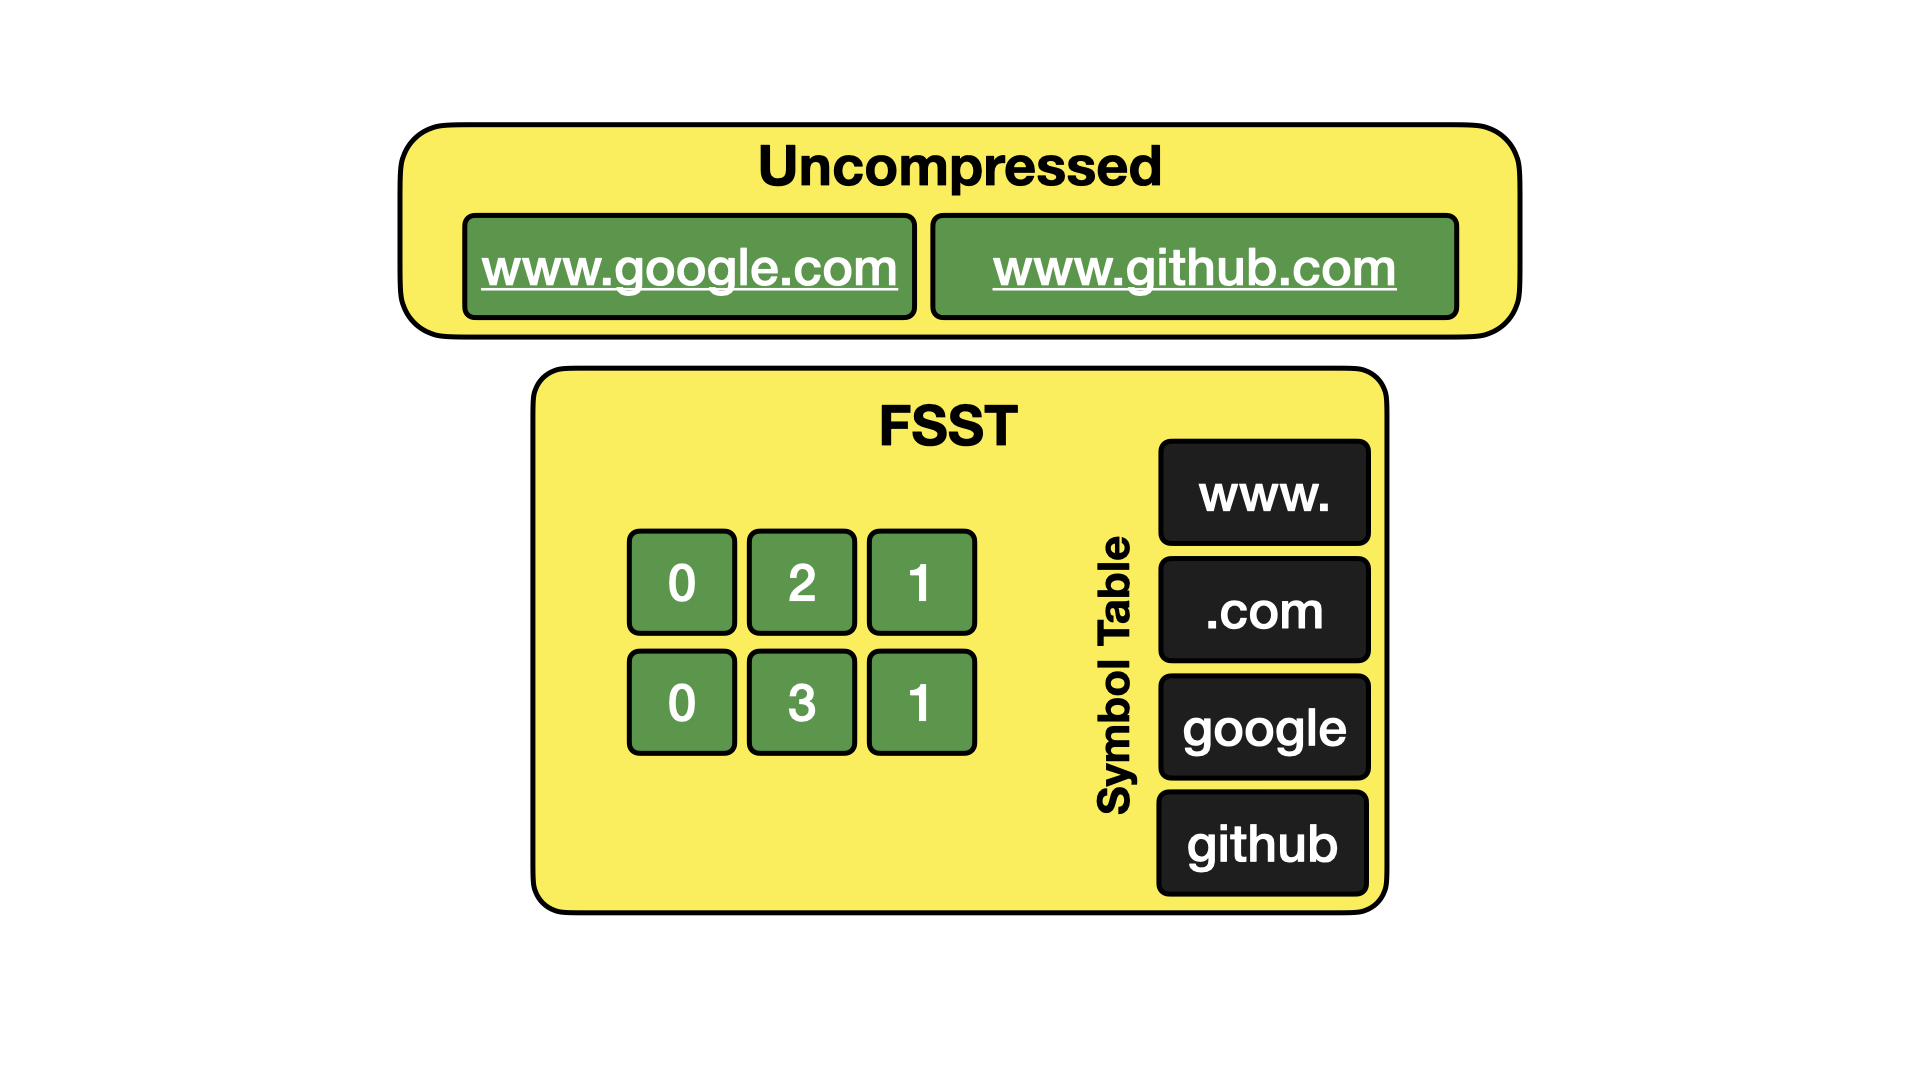
\includegraphics[width=.8\linewidth]{figures/diagrams/10-3_fsst.png}
    \caption[Example of \texttt{FSST} compression]{Example of \texttt{FSST} compression \cite{Raasveldt_2022}}
    \label{fig:fsst}
\end{figure}

Note that in the previous example, the original sequence \texttt{www.google.com} is compressed as \texttt{021}. Where \texttt{0} is the identifier for \texttt{www.}, \texttt{2} identifies \texttt{google} and \texttt{1} stands for \texttt{.com}. As in the case of \textit{run-length encoding} the higher the number of repetitions, the higher the level of compression. In this case, we have successfully represented the initial string, consisting of 14 characters, with a string of only three characters, resulting in a 78\% reduction in size. Although this example is straightforward, it effectively demonstrates the underlying concept of \texttt{FSST}.

One of the greatest strengths of compression in columnar storage lies in the driver's ability to select the optimal algorithm for each scenario. Specifically, in a column-oriented store, we can leverage a variety of compression mechanisms, individually tailored to excel in compressing each column, given that we are dealing with homogeneous data. Conversely, row-oriented stores limit us to a single compression algorithm for the entire dataset. This limitation arises from the heterogeneity of the data, preventing us from employing distinct compression algorithms for each column.

\subsubsection{Data types}

According to what we have seen in the introductory lines, we are going to try and optimize as much as we can the data types that we are going to use for storing the information. For that, we are going to use the smallest data type that can hold the information we are interested in. For example, we are using \texttt{UINTEGER} for storing the IDs of the entities, as they can be represented as numbers. What's more, we are going to use the unsigned representation as we are not interested in negative numbers. This has two main benefits: first, we are going to be able to store larger numbers. To put it into perspective, the maximum value range that can be stored in a \texttt{UINTEGER} is \texttt{4,294,967,295}, whereas the largest number that can be stored in an \texttt{INTEGER} is \texttt{2,147,483,647}. This means that we can handle twice as many positive values with the same number of bits. The same reasoning applies to the rest of the data types that are going to be used. Second, we ensuring e that our data is consistent. This is, we are not going to be able to store negative numbers in a column that is supposed to store positive numbers.

From my perspective, fine-tuning the chosen data types for storing your data makes your repositories more robust. This is because you are ensuring that the data that you are working with is consistent and that you are not wasting any space. This is especially important when dealing with large amounts of data, as the storage footprint can be reduced by a factor of 2. This is the case for this project. At the beginning of it, we were using \texttt{BIGINT} for storing the IDs of the entities. However, we realized that we were wasting half of the space, as the IDs are always positive. For that, we decided to switch to \texttt{UINTEGER}. Summing up, we moved from an 8-byte integer to a 4-byte representation, which means that we were able to store twice as many IDs with the same number of bits. This also leads to fitting more data both in memory and in the cache, which is going to be beneficial for the second part of the tool, where the graph is going to be built.

Regarding the encoding of IDs, we had two main possibilities. First, we could have used the string representation, which is the one that is employed in the JSON dump. However, we decided to go for the numeric representation as it is more compact. This is because the string representation of the IDs is composed of a prefix followed by a sequence of numbers. For example, the string representation of the ID \texttt{Q92743} is \texttt{"Q92743"}, whereas the numeric representation of the same ID is \texttt{92743}. As we are using a \texttt{UINTEGER} for representing the numeric data, only 4 bytes per row are needed. However, a string takes 1 byte per character. Thus, according to the previous example, we would need 6 bytes for encoding the string representation of the ID, while only 4 are required for the numeric representation. In this example, 2 bytes are saved. Note that this scales for even larger IDs.

The problem is that things are not as simple as they seem at first glance. Wikidata IDs not only are numeric identifiers, but they also annotate the type of the item they support: Entities, Properties, Lexemes, Forms and Senses. Thus, we need a way for encoding and decoding this information. For this purpose, what we have done is diving the address space of the IDs into 5 different ranges, one for each type. The ranges have a length of 1 hundred million, except for Forms and Senses, each of them has half that size, which is more than enough for representing the different Wikidata IDs. See the code below for more information.

\begin{code}[The From trait implementation for the ID type]
    \inputminted{rust}{code/listings/10-1_ids.rs}
\end{code}

It is worth mentioning that the most powerful thing about the \texttt{From} \texttt{trait} in Rust is that it allows us to not only convert from one type to another; but in the opposite direction too. This is, it automatically implements the \texttt{Into} \texttt{trait} thanks to the blanket implementation in the standard library. Hence, now we can convert from \texttt{u32} to \texttt{Id} and vice-versa. That is, we can serialize and deserialize the IDs transparently.

\subsubsection{Memory allocator}

A memory allocator is a software component that manages the allocation and deallocation of memory in a program. Its primary goal is to efficiently use available memory by keeping track of allocated and free memory blocks. Allocators work with a memory region called the heap, where objects are dynamically allocated. When a program requests memory, the allocator finds a free block, marks it as allocated, and returns a pointer to the program. Deallocation involves marking the block as free.

Memory allocators can employ various algorithms and data structures to manage memory efficiently. They may use techniques like linked lists, bitmaps, or binary trees to track the state of memory blocks and quickly find free blocks for allocation. Additionally, advanced allocators may employ strategies like caching, thread-specific allocation pools, or memory reuse techniques to optimize performance and reduce overhead.

Different programming languages and platforms often provide default memory allocators, but developers can also choose alternative allocators, such as \texttt{Jemalloc}, for specific optimizations or requirements. By selecting an appropriate memory allocator, developers can improve memory usage, minimize fragmentation, enhance performance, and cater to the specific needs of their applications.

\texttt{Jemalloc} is a memory allocator that can be used in Rust binary projects to optimize memory management and improve application performance. When a program allocates and deallocates memory frequently, the default memory allocator in Rust (system allocator) can introduce overhead due to its design choices and trade-offs, as it is optimized for general-purpose use and targets several different platforms and environments. However, \texttt{Jemalloc} is a specialized allocator that aims for reducing memory fragmentation. When memory allocation and deallocation are frequent, small gaps tend to form between allocated memory blocks. These gaps are called fragmentation and can lead to inefficient memory usage. Note that in the context of Big data applications, efficient memory management may improve the performance of the solution by orders of magnitude. \texttt{Jemalloc} uses a technique called \textit{arena-based memory allocation} to reduce fragmentation and improve performance. It also uses a \textit{thread-specific caching} strategy to reduce the overhead of synchronization and improve performance in multi-threaded applications. As we will see in the next chapter, one of the main optimizations that we will implement is writing our solution in a multi-threaded fashion. Thus, using \texttt{Jemalloc} is going to be beneficial for us. Lastly, note that \texttt{Jemalloc} is a platform-specific allocator, which means that it is only available on Linux and macOS. However, this allows it to use platform-specific features to improve performance.

For us to use \texttt{Jemalloc}, we need to add the following lines to the \texttt{Cargo.toml} file.

\begin{code}[The Cargo.toml file for using Jemalloc]
    \inputminted{toml}{code/listings/10-2_cargo.toml}
\end{code}

What's more, we need to use it as the default allocator for our application. For this, we need to add the following lines to the \texttt{main.rs} file. Recall that the memory allocator should be set in the main function of the application before any other code is executed. This is because the allocator is a global resource, and it is not possible to change it once it has been set. Note that in the case of libraries, changing the allocator won't have any impact, as it is the responsibility of the application to do so.

\begin{code}[The main.rs file for using Jemalloc]
    \inputminted{rust}{code/listings/10-3_main.rs}
\end{code}

\subsubsection{Compiler options}

During the development stage, Rust applications are constructed using the \texttt{dev} flag, which compiles the program without applying any optimizations. By default, the \texttt{opt-level} is set to 0 in order to facilitate easy debugging. The compilation process focuses on detecting potential panics or errors during execution. However, when preparing the tool for deployment, it is recommended to utilize the \texttt{release} profile, which leverages maximum optimization. The \texttt{opt-level} is set to 3 by default, enabling beneficial optimizations. Functions are rewritten to execute faster, incorporating techniques like inlining that make them harder to debug. Additionally, the \texttt{LTO} (Link Time Optimization) is enabled, allowing the compiler to optimize code across different compilation units. This is particularly significant when working with various modules and crates. By utilizing the \texttt{LTO} build, we aim to discover optimizations that span across different dependencies and crates, although this may result in slower compilation times. The \texttt{Cargo.toml} file specifies the release profile as follows:

\begin{code}[The Cargo.toml file for using the release profile]
    \inputminted{toml}{code/listings/10-4_cargo.toml}
\end{code}

\subsubsection{Targeting the right Platform}

Targeting the right platform in Rust is essential for optimizing performance. By specifically focusing on the platform, you can leverage architecture-specific optimizations, taking advantage of specialized hardware accelerators and maximizing the efficiency of memory management. Rust's compiler offers optimization flags and the ability to link with platform-specific libraries, enabling tailored performance enhancements. This approach ensures compatibility with the target platform's operating system, architecture, and hardware configurations, ultimately resulting in improved performance and efficiency for Rust applications. For us to target the right platform, we need to add the following lines to the \texttt{.cargo/config} file.

\begin{code}[The .cargo/config file for targeting the right platform]
    \inputminted{toml}{code/listings/10-5_config}
\end{code}

\subsection{Quality assurance}

In the following subsections, we are going to discuss the different quality assurance mechanisms that are going to be used for the development of the tool. The idea is to ensure that it is robust and that can be used in production environments. For that, we are going to use a combination of different techniques, such as version control, documentation, testing, continuous integration and continuous deployment. Note that the tool is going to be open-source, which means that the community will be able to contribute to the project. This is going to be beneficial for it as it will allow us to build a more robust tool, as third parties can examine the product we ship. Lastly, note that we are going to use this same methodology for the development of the other tools that are going developed in this thesis.

\subsubsection{Version control}

Recall that we are building an open-source solution. For this, we are going to use Git as our version control system. The idea is to use GitHub as our remote repository. This will allow us to have a public warehouse where the community can contribute to the project. Moreover, we are going to use Git tags for the versioning, letting us have a clear understanding of the different versions of the tool. For instance, we are using the \texttt{v0.0.1} tag for the first version. Subsequent versions will be annotated with a \texttt{v0.0.x} tag. What's more, for the sake of simplicity, we are going to use \textit{stable mainline} as our branching strategy for the development of the tool. This means that we are going to have a \texttt{main} branch where the latest stable version is going to be stored. The idea is to have a \texttt{dev} branch where most of the development process is going to take place. Once we have a stable version, we will merge it into the \texttt{main} branch. Note that this is a simple branching strategy that will work just fine for the development of this project as I am the sole developer. However, for larger projects, a more complex branching strategy should be considered.

\subsubsection{Documentation}

Having that said, writing good documentation is essential for the development of a robust project. For that, we are going to use Rust's documentation tool, namely, \texttt{rustdoc}. The idea is to document the different \texttt{functions}, \texttt{structs}, \texttt{traits} and \texttt{modules} of the tool so that the community can have a clear understanding of its API. Moreover, we are going to use \texttt{rustdoc}'s \texttt{doc-tests} feature for writing tests in the documentation. Putting this all together, the whole documentation will be deployed to \texttt{docs-rs}\footnote{\url{https://docs.rs/wikidata-rs/latest/wikidata_rs/}}.

\subsubsection{Testing}

The idea is to have a robust tool that can be used in production environments. For that, we are going to use Rust's testing framework, namely, \texttt{cargo test}. The idea is to write unit tests for the different functions of the tool. Something neat about \textit{unit testing} in Rust is that it encourages developers to write tests in the same file\footnote{\url{https://github.com/angelip2303/pregel-rs/blob/main/src/pregel.rs\#L873}} as the code. This is a good practice as it allows us to have a clear understanding of the different tests that are being run.

\subsubsection{Continuous integration and continuous deployment}

The result of combining the previous techniques is a robust tool that can be used in production environments. However, we are going to take it one step further by using continuous integration and continuous deployment. The idea is to make use of GitHub Actions. This is, having an Action that will run the tests of the tool every time a new commit is pushed to the repository's \texttt{main} branch. This will allow us to have a clear understanding of the state of the tool. Moreover, we are going to have another GitHub Action that will be in charge of deploying the tool to the \texttt{crates.io}\footnote{\url{https://crates.io}} platform so that other developers can use it in their projects.

\subsection{User manual}

\subsubsection{Installation}

Make sure that you install the latest stable version of Rust\footnote{\url{https://www.rust-lang.org/}}; that is, as of May 5th, version 1.69 or later, then run:

\begin{minted}{shell-session}
$ cargo install wd2duckdb
\end{minted}

This will compile \texttt{wd2duckdb} for your native architecture, increasing the performance. Recall the optimizations that we have discussed in the previous section. However, if you want to compile it for a different architecture, you can use the \texttt{--target} flag.

\subsubsection{Usage}

Several command-line options are available to customize the behavior of \texttt{wd2duckdb}. The following is a list of the most important ones:

\begin{enumerate}
    \item \texttt{--json}: The path to the \texttt{.json} file that contains the Wikidata dump. This is a required argument.
    \item \texttt{--database}: The path to the DuckDB database file. This is a required argument.
\end{enumerate}

The following is an example of how to use the tool:

\begin{minted}{shell-session}
$ wd2duckdb --json <JSON_FILE> --database <DUCKDB_FILE>
\end{minted}

Use \texttt{-} as \texttt{<JSON\_FILE>} to read from standard input instead of from a file. This makes it possible to build a pipeline that processes JSON data as it is being decompressed, without having to decompress the full dump to disk. In the case of a \texttt{.bz2} file, you can use the following instruction:

\begin{minted}{shell-session}
$ bzcat latest-all.json.bz2 | wd2duckdb --json - --database <DUCKDB_FILE>
\end{minted}

In case of a \texttt{.gz} compressed file, the following is required:

\begin{minted}{shell-session}
$ gunzip latest-all.json.gz | wd2duckdb --json - --database <DUCKDB_FILE>
\end{minted}

In case you want to write changes directly to the standard output; that is, without creating a file for the uncompressed \texttt{.json}, you can do the following. Note the use of the \texttt{-c} flag in \texttt{gunzip}:

\begin{minted}{shell-session}
$ gunzip -c latest-all.json.gz | wd2duckdb --json - --database <DUCKDB_FILE>
\end{minted}

If you are working with large dumps where the uncompressed \texttt{.json} file size is in the order of \texttt{Terabytes}, it is best to choose the last option. The \texttt{.duckdb} file, which is more memory-efficient, may thus be created immediately. This is because the \texttt{.json} file is not stored in memory, but rather, it is streamed from the standard input.

\subsection{Known limitations}

During the development of our tool, we encountered a limitation related to the \texttt{wikidata}\footnote{\url{https://crates.io/crates/wikidata}} library, which cannot parse JSON dumps before 2017-08-21. This limitation is shared by other tools aiming to import Wikidata dumps\footnote{\url{https://github.com/usc-isi-i2/kgtk/issues/108}}, as mentioned in an issue reported on GitHub. Although the specific reasons for this limitation are not well-documented in Wikidata's developer portal, we have found some clues that may provide insights into the possible cause\footnote{\url{https://github.com/usc-isi-i2/kgtk/issues/272\#issuecomment-748350311}}. The limitation arises from the way references to properties and values are serialized in the dumps. Recall figure \ref{fig:wikibaseStatement}, where we can see that the Statement has a \texttt{mainSnak}, which is the main claim of the statement. Before the mentioned date, the referencing was done using only the numeric identifier (\texttt{numeric-id}) instead of the full identifier expected by the library. For example, the property \texttt{P31} was referenced as \texttt{\{numeric-id: 31\}} instead of \texttt{\{numeric-id: 31, id: "P31"\}}. Hence, the library fails to parse the Wikidata entities. Even if we will continue monitoring the development of the \texttt{wikidata} library to see if this issue is resolved in future updates, fixing it ourselves is challenging and not a priority for our tool's development at the moment, as we can work with dumps from 2017-08-21 onwards.

\chapter{A tool for validating Knowledge Graphs}
\label{chapter:pschema}
\epigraph{\textit{Logic is the foundation of the certainty of all the Knowledge we acquire.}}{-- \textup{Leonhard Euler}}

The main goal of this thesis is to create a tool capable of creating subsets out of a Knowledge graph. In this chapter, we will explore the possibility of implementing the Pregel framework in Rust, as well as a novel approach to the problem of Knowledge graph validation.

\section{Pregel-rs}



\section{PSchema-rs}

\subsubsection{Optimizations}

\paragraph{Parallelization}

The first optimization that we are going to consider is parallelization. The idea is to split the DuckDB dump into several chunks and then parse each of the chunks in parallel. This is going to be done by the first component of the tool. For this purpose, we are using \texttt{rayon}\footnote{\url{https://github.com/rayon-rs/rayon}}. This library is a data-parallelism API for Rust that provides several parallel iterators. Hence, we are using one to traverse the database in parallel. This can be done because each of the lines of the chunks of the dump is independent of each other. Thus, we can parse each of the entities in parallel without having to worry about synchronization issues. What's more, the \texttt{rayon} library is going to take care of the load balancing for us. This means that we do not have to worry about splitting the DuckDB dump into chunks of equal size. Lastly, \texttt{rayon} is also in charge of handling the thread pool for us and caring about the data-races that might arise.

What I like the most about \texttt{rayon} is the ease of transforming a sequential iterator into a parallel one. Let's have a look at an example of how this can be done:

\begin{minted}{rust}
    let lines = BufReader::new(file).lines();
    let lines = lines.into_par_iter();
\end{minted}

Whereas the first line creates a sequential iterator, the second one transforms it into a parallel one. This is done by calling the \texttt{into\_par\_iter} method on the iterator. Even if we have just shown a simple example, the actual solution is not far from what we have just shown above. See the code in the repository\footnote{\url{https://github.com/angelip2303/pschema-rs/blob/e51a24c194184db5f71bacb5289b8af55caa5146/src/backends/duckdb.rs\#L64}} for a more detailed example:

\begin{minted}{rust}
    let batches: Vec<RecordBatch> = match statement.query_arrow([]) {
        Ok(arrow) => arrow.collect(),
        Err(_) => return Err(String::from("Error executing the Arrow query")),
    };

    batches
        .into_par_iter()
        .map(|batch| {
            // Processing goes here...
        });
\end{minted}

\part{Project Synthesis}

\chapter{Experimental Procedure}
\label{chapter:experiment}
\epigraph{\textit{No amount of experimentation can ever prove me right; a single experiment can prove me wrong.}}{-- \textup{Albert Einstein}}

\section{Methodology}

For us to evaluate the performance of our proposed method, we need to compare it with the state-of-the-art tools we showed in Chapter \ref{chapter:related}. For us to do so, we need to have a set of experiments that we can run on the same software environment. We also need to have a bunch of datasets that we can use to run the experiments. In this chapter, we will describe the methodology we used to conduct the experiments and the datasets we used to run them. For us to achieve this, we will answer the questions posed in Chapter \ref{chapter:intro}, namely, the project goals (see section \ref{section:objectives}).

\begin{enumerate}
    \itemsep0.5em
    \item To evaluate how the \textit{subsetting} tool has been improved, we need to run the \textit{subsetting} tool on the same software environment as the one used in the original paper. We will use the \textit{ETL} tool to compress the Wikidata JSON dump to a size that is manageable for the \textit{Pregel} algorithm. This is, we will try to tell if the tool has been improved in terms of the hardware needed to run it. Recall that for Labra's \cite{https://doi.org/10.48550/arxiv.2110.11709} solution to work, a costly machine with 4TB of RAM is required. We will verify if our solution can run on commodity hardware.
    \item To evaluate how the \textit{subsetting} tool has been improved, we need to measure the time it takes to subset the Wikidata JSON dump. We will compare the time it takes to subset the Wikidata JSON dump with the time it takes to subset the Wikidata JSON dump using the original tool.
    \item To evaluate how the \textit{subsetting} tool has been improved, we will try to subset other RDF datasets, apart from the Wikidata JSON dump. This is, we will try to tell if the tool is generic enough to subset other RDF Knowledge graphs.
\end{enumerate}

\section{Hardware}

For us to run the experiments, we need to have a machine with enough resources to run them. Hence, we will use a machine proprietary of the \textit{Web Semantic Research Group} (WESO) of the \textit{University of Oviedo}. The machine has the following specifications:

\begin{itemize}
    \itemsep0.5em
    \item \textbf{CPU}: Intel(R) Xeon(R) Silver 4214 CPU @ 2.20GHz (12 cores and 24 threads)
    \item \textbf{RAM}: 40GB
    \item \textbf{OS}: Ubuntu 20.04.3 LTS
\end{itemize}

\section{Datasets}

To test the above questions, we will use two types of datasets, namely, Wikidata JSON dumps and RDF datasets. We will use the Wikidata JSON dumps from 2017-08-21 to test the \textit{ETL} tool, and we will use both for the \textit{subsetting} tool. For us to compare our solution with the original one, we will use the same Wikidata JSON dump used in the original paper.

\chapter{Results and Analysis}
\label{chapter:results}
\epigraph{\textit{80\% of a piece of software can be written in 20\% of the total allocated time. Conversely, the hardest 20\% of the code takes 80\% of the time.}}{-- \textup{Roger S. Pressman}}

\section{\texttt{wd2duckdb}}

As we have seen in the previous chapter, the \texttt{wd2duckdb} tool is analyzed thoroughly for us to understand how it performs and what can be done to improve it. In this section, we will present the execution times of the tool provided several configurations. What we want to see is how the tool performs with different optimizations enabled and how it compares to the original version of the tool. As such, we will prove that the optimizations we have implemented are indeed useful and that they improve the performance of the tool. Recall that the optimizations that we have implemented were described in section \ref{section:optimizations}.

As can be seen in Figure \ref{fig:wd2duckdb}, the optimizations that we have implemented improve the performance of the tool. This is something that was expected before running the tests; however, the results obtained prove to be a worthy improvement. Note that for us to test the performance of the tool, we have used the same Wikidata dump for all the tests. The idea is to create 8 different databases each three times larger than the previous one. This, we have increased the number of Wikidata entities by a factor of 3 each time, starting from 10 thousand items to 21.87 million elements. This is, values in the abscissa axis
can be obtained through the following representation: $10,000 \cdot 3^n, n \in [0, 7]$. For us to fit such a big range of values in a single graph, we have used a logarithmic scale for the x-axis. This way, we can see the results of the tests in a single graph. Note that for the y-axis, we have used a linear scale, as the values are not that big, ranging from $0$ to $4,000$ and $40,000$ seconds, respectively, modeling the time it took to generate the database. This is said to be a \textit{semi-logarithmic} plot. To put it all together, we have used this type of representation to manage to test the tool with a wide range of values, and still, be able to see the results in a single graph.

For us to understand the values better, let me show them in a table, and then, we will comment on them in detail. Table \ref{table:wd2duckdb} shows the time it took to create the database with the different optimizations enabled and disabled.

\begin{table}[ht]
    \centering
    \begin{tabular}{|c|c|c|c|c|c|c|c|c|}
        \hline
        \rowcolor[HTML]{EFEFEF}
        \cellcolor[HTML]{C0C0C0}\textbf{N}               & \textit{0} & \textit{1} & \textit{2} & \textit{3} & \textit{4} & \textit{5} & \textit{6} & \textit{7} \\ \hline
        \cellcolor[HTML]{C0C0C0}\textbf{Optimizations}   & 4.56       & 11.05      & 26.36      & 54.87      & 112.30     & 250.86     & 1,349.10   & 3,730.33   \\ \hline
        \cellcolor[HTML]{C0C0C0}\textbf{No Optimization} & 40.18      & 99.52      & 243.64     & 514.68     & 1,081.64   & 2,566.25   & 13,157.18  & 37,340.60  \\ \hline
    \end{tabular}
    \caption{Time to create the database with \texttt{wd2duckdb}}
    \label{table:wd2duckdb}
\end{table}

As can be seen, the time it takes \texttt{wd2duckdb} to process the dumps grows at a linear rate. What's more, we can see that the speedup in the execution time is almost 10. Let me first calculate this value, and then, we will comment on the results. Having ${Time_{DEV}}_i$ the $i^{th}$ execution time of the tool in developer mode, that is, with no optimization enabled, and ${Time_{OPT}}_j$ the $j^{th}$ execution time of the tool in release mode, that is, with all the optimizations enabled. The speedup is calculated as follows:

\begin{equation}
    \text{Speedup} = \frac{\overline{Time_{DEV}}}{\overline{Time_{OPT}}} = \frac{\sum_{i=0}^{7}t_i}{\sum_{j=0}^{7}t_j} = \frac{40.18 + \cdots + 37,340.60}{4.56 + \cdots + 3,730.33} = \frac{55,043.70}{5,539.43} = 9.94
\end{equation}

\begin{figure}[p]
    \begin{subfigure}{0.49\textwidth}
        \centering
        \includestandalone[width=\textwidth,height=8cm]{diagrams/13-1_wd2duckdbOPT}
        \caption{Having all the optimizations enabled}
    \end{subfigure}%
    \hfill
    \begin{subfigure}{0.49\textwidth}
        \centering
        \includestandalone[width=\textwidth,height=8cm]{diagrams/13-2_wd2duckdbDEV}
        \caption{Having no optimization enabled}
    \end{subfigure}%
    \vspace*{1em}
    \begin{subfigure}{\textwidth}
        \centering
        \includestandalone[width=\textwidth]{diagrams/13-3_wd2duckdbBAR}
        \caption{Comparison between the two options: with and without optimizations}
    \end{subfigure}
    \caption{Time to create the database with \texttt{wd2duckdb}}
    \label{fig:wd2duckdb}
\end{figure}

\section{\texttt{pschema-rs}}

\begin{table}[ht]
    \centering
    \begin{tabular}{|
            >{\columncolor[HTML]{C0C0C0}}c |c|c|c|}
        \hline
        \textbf{N}          & \cellcolor[HTML]{EFEFEF}\textit{0} & \cellcolor[HTML]{EFEFEF}\textit{1} & \cellcolor[HTML]{EFEFEF}\textit{2} \\ \hline
        \textbf{pschema-rs} & 5,014.34                           & 4,995.30                           & 4,996.04                           \\ \hline
        \textbf{wdsub}      & 5,090.01                           & 5,064.14                           & 5,071.09                           \\ \hline
    \end{tabular}
    \caption{Time to create the \textit{subsets} of Wikidata with \texttt{pschema-rs} and \texttt{wdsub}}
\end{table}

\begin{equation}
    \text{Speedup} = \frac{\overline{Time_{wdsub}}}{\overline{Time_{pschema-rs}}} = \frac{\sum_{i=0}^{2}t_i}{\sum_{j=0}^{2}t_j} = \frac{5,090.01 + \cdots + 5,071.09}{5,014.34 + \cdots + 4,996.04} = \frac{15,225.28}{15,005.69} = 1.01
\end{equation}

\begin{figure}[p]
    \begin{subfigure}{\textwidth}
        \centering
        \includestandalone[width=\textwidth,height=6cm]{diagrams/13-4_pschemaN}
        \caption{Modifying the number of Wikidata Entities}
    \end{subfigure}%
    \vspace*{1em}
    \begin{subfigure}{\textwidth}
        \centering
        \includestandalone[width=\textwidth,height=6cm]{diagrams/13-5_pschemaDEPTH}
        \caption{Modifying the depth of the \texttt{ShEx} tree}
    \end{subfigure}%
    \vspace*{1em}
    \begin{subfigure}{\textwidth}
        \centering
        \includestandalone[width=\textwidth,height=6cm]{diagrams/13-6_pschemaBREADTH}
        \caption{Modifying the breadth of the \texttt{ShEx} tree}
    \end{subfigure}
    \caption{Time to create the \textit{subsets} of Wikidata with \texttt{pschema-rs}}
\end{figure}

\chapter{Planning and Budget}
\label{chapter:planning}
\epigraph{\textit{Give me six hours to chop down a tree and I will spend the first four sharpening the axe.}}{-- \textup{Abraham Lincoln}}

\section{Planning}

This project's planning was divided into four main phases: the first one was the \textbf{research phase}, where the state of the art was studied and the main concepts were understood; the second one was the \textbf{development phase}, where the main focus was to develop the project's solution; to continue, the \textbf{writing phase} was the period at which the thesis was written. Lastly, the last part of this project is the \textbf{defense of the work phase}, where the thesis is presented and defended. Thus, we can see the project's timeline in \ref{fig:summary_timeline}, for a more detailed description, see Figure \ref{fig:timeline} and Table \ref{tab:timeline}.

\begin{figure}[ht]
    \centering
    \includestandalone[width=1\textwidth]{diagrams/14-2_summary}
    \caption{Project timeline highlighting the most important reached milestones}
    \label{fig:summary_timeline}
\end{figure}

\subsection{Research phase}

The research phase was divided into two main parts: the first one was the \textbf{research of the state of the art}, where the main concepts were studied and understood; the second one was the \textbf{research of the technologies}, where the technologies that were going to be used in the project were analyzed. To be fair, part of this phase was done during the development phase, as we changed the technologies that were going to be used in the project. However, the main concepts were already understood, so the research on the technologies was not that hard. Hence, we can say that the research phase ended when the development phase started.

\subsection{Development phase}

The development phase was divided into three main parts: the first one was the \textbf{development of DataFrame-based solution}, where we tried to develop a solution based on DataFrames. As have already discussed, the outcome of this part was not as expected, so we had to change the approach; the second one was the \textbf{development of the ETL pipeline}, where we developed the \texttt{wd2duckdb} tool; the third one was the \textbf{development of the Pregel algorithm}, where we developed the \texttt{pschema-rs} tool.

\subsection{Writing phase}

The writing phase was divided into two main parts: the first one was the \textbf{literature review}, where the state of the art was studied and written; the second one was the \textbf{thesis}, where the thesis was written. The first part was done during the research phase; for the sake of simplicity, we will consider that the \textit{literature review} stage is part of the \textit{research phase}. Hence, the writing phase is only composed of the \textit{thesis} stage, where I wrote the part of the thesis that is created entirely by me.

\subsection{Defense of the work phase}

The defense of the work phase was divided into two main parts: the first one was the \textbf{presentation of the thesis}, where the slides and the presentation were created; the second one was the \textbf{defense of the thesis}, where the thesis is going to be presented and defended. This part has not been done yet; however, it is already planned.

\section{Budget}

Note that part of this project was done during an internship at \textit{WESO}. Hence, the budget for this project is going to be calculated based on the rate that the \textit{University of Oviedo} pays to its interns\footnote{\url{https://www.funiovi.org/estudiantes/practicas}}. Provided a 20 hours per week internship, the maximum wage is 400€ per month. Hence, given that a work month has 4.33 weeks, the hourly rate is 4.61€. This rate is going to be used to calculate the budget of this project.

\begin{figure}[p]
    \centering
    \includestandalone[width=1\textwidth]{diagrams/14-1_timeline}
    \caption{Project timeline highlighting all the reached milestones}
    \label{fig:timeline}
\end{figure}

\begin{table}[p]
    \centering
    \documentclass{standalone}
\usepackage[table,xcdraw]{xcolor}
\usepackage{varioref,multicol}
\usepackage{hyperref}  
\begin{document}
\begin{tabular}{|r|llll|}
    \hline
    \rowcolor[HTML]{C0C0C0}
    \multicolumn{1}{|c|}{\cellcolor[HTML]{C0C0C0}\textbf{ID}}     & \multicolumn{1}{c|}{\cellcolor[HTML]{C0C0C0}\textbf{Task name}} & \multicolumn{1}{c|}{\cellcolor[HTML]{C0C0C0}\textbf{Duration}} & \multicolumn{1}{c|}{\cellcolor[HTML]{C0C0C0}\textbf{Start}} & \multicolumn{1}{c|}{\cellcolor[HTML]{C0C0C0}\textbf{Finish}} \\ \hline
    \textbf{1}                                                    & \multicolumn{4}{c|}{\textit{Meetings}}                                                                                                                                                                                                                        \\ \hline
    1.1                                                           & \multicolumn{1}{l|}{Project's first meeting}                    & \multicolumn{1}{l|}{1 hour}                                    & \multicolumn{1}{l|}{Fri 16 September, 2022}                 & Fri 16 September, 2022                                       \\ \hline
    1.2                                                           & \multicolumn{1}{l|}{Project's second meeting}                   & \multicolumn{1}{l|}{2.5 hours}                                 & \multicolumn{1}{l|}{Thu 29 September, 2022}                 & Thu 29 September, 2022                                       \\ \hline
    1.3                                                           & \multicolumn{1}{l|}{Project's third meeting}                    & \multicolumn{1}{l|}{2 hours}                                   & \multicolumn{1}{l|}{Mon 20 February, 2023}                  & Mon 20 February, 2023                                        \\ \hline
    \textbf{2}                                                    & \multicolumn{4}{c|}{\textit{Literature Review}}                                                                                                                                                                                                               \\ \hline
    2.1                                                           & \multicolumn{1}{l|}{Knowledge graphs}                           & \multicolumn{1}{l|}{5 hours}                                   & \multicolumn{1}{l|}{Thu 29 September, 2022}                 & Fri 30 September, 2022                                       \\ \hline
    2.2                                                           & \multicolumn{1}{l|}{Wikibase graphs}                            & \multicolumn{1}{l|}{10 hours}                                  & \multicolumn{1}{l|}{Fri 30 September, 2022}                 & Sat 15 October, 2022                                         \\ \hline
    2.3                                                           & \multicolumn{1}{l|}{Knowledge Graph validation}                 & \multicolumn{1}{l|}{7 hours}                                   & \multicolumn{1}{l|}{Sat 29 October, 2022}                   & Sat 5 November, 2022                                         \\ \hline
    2.4                                                           & \multicolumn{1}{l|}{Knowledge Graph Subsetting}                 & \multicolumn{1}{l|}{0.5 hours}                                 & \multicolumn{1}{l|}{Mon 7 November, 2022}                   & Mon 7 November, 2022                                         \\ \hline
    2.5                                                           & \multicolumn{1}{l|}{MapReduce}                                  & \multicolumn{1}{l|}{3 hours}                                   & \multicolumn{1}{l|}{Tue 4 October, 2022}                    & Tue 4 October, 2022                                          \\ \hline
    2.6                                                           & \multicolumn{1}{l|}{Pregel system}                              & \multicolumn{1}{l|}{6 hours}                                   & \multicolumn{1}{l|}{Tue 4 October, 2022}                    & Thu 6 October, 2022                                          \\ \hline
    \textbf{3}                                                    & \multicolumn{4}{c|}{\textit{Dissertation Document}}                                                                                                                                                                                                           \\ \hline
    3.1                                                           & \multicolumn{1}{l|}{Introduction}                               & \multicolumn{1}{l|}{5 hours}                                   & \multicolumn{1}{l|}{Wed 9 November, 2022}                   &                                                              \\ \hline
    3.2                                                           & \multicolumn{1}{l|}{Related Work}                               & \multicolumn{1}{l|}{3 hours}                                   & \multicolumn{1}{l|}{Fri 11 November, 2022}                  &                                                              \\ \hline
    3.3                                                           & \multicolumn{1}{l|}{Theoretical Background}                     & \multicolumn{1}{l|}{45 hours}                                  & \multicolumn{1}{l|}{Thu 29 September, 2022}                 &                                                              \\ \hline
    3.4                                                           & \multicolumn{1}{l|}{Analysis of the Initial solution}           & \multicolumn{1}{l|}{10 hours}                                  & \multicolumn{1}{l|}{Fri 11 November, 2022}                  &                                                              \\ \hline
    3.5                                                           & \multicolumn{1}{l|}{The DataFrame-based solution}               & \multicolumn{1}{l|}{10 hours}                                  & \multicolumn{1}{l|}{Fri 11 November, 2022}                  &                                                              \\ \hline
    3.6                                                           & \multicolumn{1}{l|}{Analysis of the Rust solution}              & \multicolumn{1}{l|}{10 hours}                                  & \multicolumn{1}{l|}{Fri 11 November, 2022}                  &                                                              \\ \hline
    3.7                                                           & \multicolumn{1}{l|}{The ETL pipeline}                           & \multicolumn{1}{l|}{10 hours}                                  & \multicolumn{1}{l|}{Fri 11 November, 2022}                  &                                                              \\ \hline
    3.8                                                           & \multicolumn{1}{l|}{The subsetting tool}                        & \multicolumn{1}{l|}{10 hours}                                  & \multicolumn{1}{l|}{Fri 11 November, 2022}                  &                                                              \\ \hline
    3.9                                                           & \multicolumn{1}{l|}{Experimental Procedure}                     & \multicolumn{1}{l|}{}                                          & \multicolumn{1}{l|}{}                                       &                                                              \\ \hline
    3.10                                                          & \multicolumn{1}{l|}{Results and Analysis}                       & \multicolumn{1}{l|}{}                                          & \multicolumn{1}{l|}{}                                       &                                                              \\ \hline
    3.11                                                          & \multicolumn{1}{l|}{Planning and Budget}                        & \multicolumn{1}{l|}{}                                          & \multicolumn{1}{l|}{Thu 20 October, 2022}                   &                                                              \\ \hline
    3.12                                                          & \multicolumn{1}{l|}{Conclusions}                                & \multicolumn{1}{l|}{}                                          & \multicolumn{1}{l|}{}                                       &                                                              \\ \hline
    \textbf{4}                                                    & \multicolumn{4}{c|}{\textit{Proposed Solution Development}}                                                                                                                                                                                                   \\ \hline
    4.1                                                           & \multicolumn{1}{l|}{The DataFrame-based solution}               & \multicolumn{1}{l|}{30 hours}                                  & \multicolumn{1}{l|}{Sun 29 January, 2023}                   & Mon 20 February, 2023                                        \\ \hline
    4.2                                                           & \multicolumn{1}{l|}{\texttt{wd2duckdb}}                         & \multicolumn{1}{l|}{}                                          & \multicolumn{1}{l|}{Tue 21 February, 2023}                  &                                                              \\ \hline
    4.3                                                           & \multicolumn{1}{l|}{\texttt{pregel-rs}}                         & \multicolumn{1}{l|}{}                                          & \multicolumn{1}{l|}{Tue 21 February, 2023}                  &                                                              \\ \hline
    4.4                                                           & \multicolumn{1}{l|}{\texttt{pschema-rs}}                        & \multicolumn{1}{l|}{}                                          & \multicolumn{1}{l|}{Tue 21 February, 2023}                  &                                                              \\ \hline
    \textbf{5}                                                    & \multicolumn{4}{c|}{\textit{Learning new technologies}}                                                                                                                                                                                                       \\ \hline
    5.1                                                           & \multicolumn{1}{l|}{Scala}                                      & \multicolumn{1}{l|}{10 hours}                                  & \multicolumn{1}{l|}{Tue 6 December, 2022}                   & Tue 27 December, 2022                                        \\ \hline
    5.2                                                           & \multicolumn{1}{l|}{Apache Spark}                               & \multicolumn{1}{l|}{5 hours}                                   & \multicolumn{1}{l|}{Thu 29 December, 2022}                  & Sat 7 January, 2023                                          \\ \hline
    5.3                                                           & \multicolumn{1}{l|}{Rust}                                       & \multicolumn{1}{l|}{5 hours}                                   & \multicolumn{1}{l|}{Tue 21 February, 2023}                  &                                                              \\ \hline
    5.4                                                           & \multicolumn{1}{l|}{DuckDB}                                     & \multicolumn{1}{l|}{5 hours}                                   & \multicolumn{1}{l|}{Tue 21 February, 2023}                  &                                                              \\ \hline
    5.5                                                           & \multicolumn{1}{l|}{Pola-rs}                                    & \multicolumn{1}{l|}{5 hours}                                   & \multicolumn{1}{l|}{Tue 21 February, 2023}                  &                                                              \\ \hline
    \textbf{6}                                                    & \multicolumn{4}{c|}{\textit{Defense of the project}}                                                                                                                                                                                                          \\ \hline
    6.1                                                           & \multicolumn{1}{l|}{Keynote document}                           & \multicolumn{1}{l|}{10 hours}                                  & \multicolumn{1}{l|}{Tue 6 December, 2022}                   & Tue 27 December, 2022                                        \\ \hline
    6.2                                                           & \multicolumn{1}{l|}{Preparation of the speech}                  & \multicolumn{1}{l|}{5 hours}                                   & \multicolumn{1}{l|}{Thu 29 December, 2022}                  & Sat 7 January, 2023                                          \\ \hline
    \multicolumn{2}{|r|}{\cellcolor[HTML]{C0C0C0}\textbf{Total:}} & \multicolumn{1}{l|}{159 hours}                                                                                                                                                                                                                                \\ \cline{1-3}
\end{tabular}
\end{document}
    \caption{Tasks planning of the project}
    \label{tab:timeline}
\end{table}

\chapter{Conclusions}
\label{chapter:conclusions}
\epigraph{\textit{The programmers of tomorrow are the wizards of the future. You're going to look like you have magic powers compared to everybody else.}}{-- \textup{Gabe Newell}}

\section{Achievements}

From June the $25^{th}$ to July the $1^{st}$, the \textit{DBCLS BioHackathon 2023} took place, this is an event focused on the standardization and interoperability of life sciences and biomedical databases, namely, Knowledge Graphs. Following this, during the event, the tool presented in this project was used to create some subsets of the \textit{Uniprot} database. Which was later published in the \textit{Zenodo} repository, and can be found in the following link: \url{https://zenodo.org/record/8086938}.

\section{Future work}

The tool presented in this project is still in its early stages, and many improvements can be made to it. Some of the most important ones are:

\begin{enumerate}
    \itemsep0.5em
    \item \textbf{Improve the performance of the tool}: The tool is still slow, and it can be improved by using a more efficient programming language, or by using a more efficient algorithm.
    \item \textbf{Add more features}: The tool can be improved by adding more features, such as the ability to create subsets of the database based on the taxonomy of the proteins.
\end{enumerate}

Apart from the improvements that I have just mentioned, several other use cases can be implemented using the tool presented in this project. Some of the most important ones are:

\section{Personal opinion}

\part{Annexes and References}

\chapterimage{img/misc/heading_bib.jpg} % Chapter heading image
\chapter{References} % Chapter heading image
\printbibliography[heading=bibempty]

\end{document}